\documentclass[9pt, aspectratio=169]{beamer}
\usetheme{Thesis}

%\usepackage[latin1]{inputenc}
\usepackage[utf8]{inputenc}
\usepackage{amsmath,amsfonts,amssymb}
\usepackage{graphics}
\usepackage{graphicx}
\usepackage{xcolor}
\usepackage{setspace}

\usepackage{multimedia}
\usepackage{media9}
\usepackage{hyperref}
\usepackage{algorithm}
\usepackage{algorithmic}
\usepackage{tikz}
\usepackage{booktabs}
\usepackage{adjustbox}
\usepackage{siunitx}
\usetikzlibrary{arrows,shapes,shadows,calc}

\setbeamertemplate{itemize/enumerate body begin}{\small}
\setbeamertemplate{itemize/enumerate subbody begin}{\footnotesize}
%\setbeamercovered{transparent}
%\setbeamercolor{block body}{bg=gray}

\setlength{\itemsep}{1ex}
\definecolor{mygreen}{RGB}{0,100,0}
\definecolor{myblue}{RGB}{42,82,190}

\newcommand{\backupbegin}{
   \newcounter{finalframe}
   \setcounter{finalframe}{\value{framenumber}}
}
\newcommand{\backupend}{
   \setcounter{framenumber}{\value{finalframe}}
}




%%%%%%%%%%%%%%%%%%%%%%%%%%%%%%%%%%%%%%%%%%%%%%%
% COLOR Command
\newcommand{\myemph}[1]{\emph{\color{emph@Thesis}#1}}
\newcommand{\mytitle}[1]{\textbf{\color{emph@Thesis}#1}}
\newcommand{\myblue}[1]{{\color{blue@Thesis}#1}}
\newcommand{\myred}[1]{{\color{red@Thesis}#1}}
%%%%%%%%%%%%%%%%%%%%%%%%%%%%%%%%%%%%%%%%%%%%%%%

\title[Control of an autonomous aerodynamic airshield for training Olympics 100m sprint athletes]
  {\Large Control of an autonomous aerodynamic airshield \\
for training Olympics 100m sprint athletes}
\author[Giulia Cutini]{Giulia Cutini}
\institute[University of Bologna]{}
\date{March 18, 2024}



\graphicspath{{figs/}}


\begin{document}
\footnotesize

%%%%%% COPERTINA %%%%%%%%%%%%%%%%%%%%%%%%%%%%%%%%%%%%%%%%%5%%%%%%%%%%%%%%%%%%%%%%
\begin{frame}[plain,noframenumbering,t]

\begin{columns}
\begin{column}{0.15\textwidth}
\begin{tikzpicture}[remember picture,overlay,opacity=0.9]
\node[anchor=north west,inner sep=0pt] at (current page.north west) {
    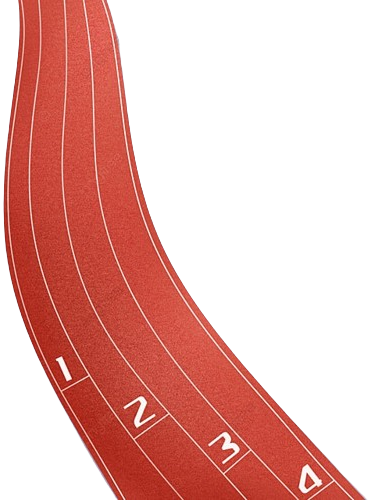
\includegraphics[height=9cm]{Pista}
};
\end{tikzpicture}
\end{column}

\begin{column}{0.85\textwidth}
\centering
\fontsize{9}{11}\selectfont
\vspace{0.8cm}
\begin{columns}
\begin{column}{1.1\textwidth}
\centering \small
\textsc{Alma Mater Studiorum Universit\`{a} di Bologna}\\
\textsc{Department of Electrical, Electronic and Information Engineering}
\\
\vspace{0.1cm}
\textsc{Master's Degree in Automation Engineering}
\end{column}
\end{columns}

\vspace{0.7cm}

\textcolor{blue@Thesis}{\bf \inserttitle}

\vspace{1cm}

\begin{columns}[t]
\begin{column}{0.5\textwidth}
    \myemph{Candidate:}
    
    \hspace{0.5cm} Giulia Cutini
\end{column}

\begin{column}{0.4\textwidth}
    \myemph{Advisor:}
    
        \hspace{0.5cm} Prof.~Giuseppe Notarstefano
        
        \vspace{.4cm}
        \myemph{Co-Advisors:}
    
        \hspace{0.5cm} Prof.~Melanie Zeilinger \\
        \hspace{0.5cm} Dr.~Andrea Carron \\
        \hspace{0.5cm} Ing.~Lorenzo Sforni
\end{column}
\end{columns}

\begin{tikzpicture}[remember picture,overlay]
\node[anchor=south east,inner sep=0pt] at (current page.south east) {
    \hspace{2cm} 
\includegraphics[height=1.5cm]{Logo_unibo}
};
\end{tikzpicture}
\begin{tikzpicture}[remember picture,overlay,opacity=0.6]
\node[anchor=south east,inner sep=0pt] at (current page.south east) {
    
\includegraphics[height=0.8cm]{Logo_ETH} \hspace{2.6cm}
};
\end{tikzpicture}

\vspace{0.8cm}
\begin{center}
\small
 \hspace{-2.5cm} \textcolor{emph@Thesis}{Bologna, 18 March 2024}
\end{center}
\end{column}
\end{columns}
\end{frame}

%%%%%% INDICE %%%%%%%%%%%%%%%%%%%%%%%%%%%%%%%%%%%%%%%%%%%%%%%%%%%%%%%%%%%%%%%%%%%
%\begin{frame}
%\frametitle{Table of Contents}
%\begin{itemize}
%	\footnotesize
%	\item[$\blacktriangleright$]<1-> Introduction
%		\begin{itemize}
%			\footnotesize
%			\setstretch{1.2}
%			\item[$\triangleright$]<1-> Motivations
%			\item[$\triangleright$]<1-> Contributions
%		\end{itemize}
%	\item[$\blacktriangleright$]<2-> Modeling of the go-kart with the airshield attached
%	\item[$\blacktriangleright$]<3-> Control design
%		\begin{itemize}
%			\footnotesize
%			\setstretch{1.2}
%			\item[$\triangleright$]<3-> Gain Scheduling Linear Quadratic Regulator
%			\item[$\triangleright$]<3-> Model Predictive Control
%			\item[$\triangleright$]<3-> Offset-free Model Predictive Control
%		\end{itemize}
%	\item[$\blacktriangleright$]<4-> Simulation test and numerical controllers comparison
%	\item[$\blacktriangleright$]<5-> Hardware-in-the-loop tests
%\end{itemize}
%\end{frame}

%%%%%% INTRODUCTION %%%%%%%%%%%%%%%%%%%%%%%%%%%%%%%%%%%%%%%%%%%%%%%%%%%%%%%%%%%%%%
\begin{frame}
\vspace{0.05cm}
\frametitle{Introduction}
\vspace{0.2cm}
\textcolor{emph@Thesis}{\textbf{\small{Motivations}}} \\
\vspace{0.2cm}

\onslide<1,2,3>In athletics, the \textbf{overspeed training} makes possible to enhance the competition performances.

\setstretch{1.3}
\onslide <1,2,3>Innovative technique: isolating the runner from the air resistance using an \textbf{airshield}.

\begin{columns}
\hspace{0.2cm}
\begin{column}{0.62\textwidth}
\vspace{0.2cm}
	\begin{center}
  		\onslide <1,2,3>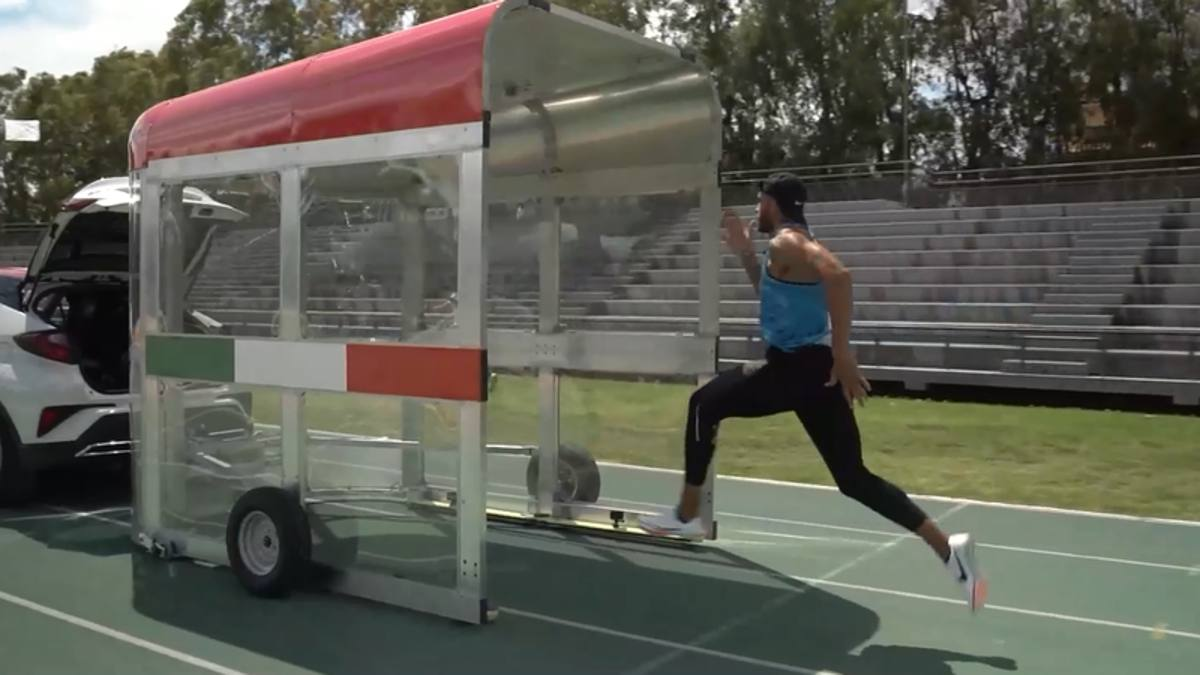
\includegraphics[width=0.48\textwidth]{Jacobs} 
		\onslide <2,3>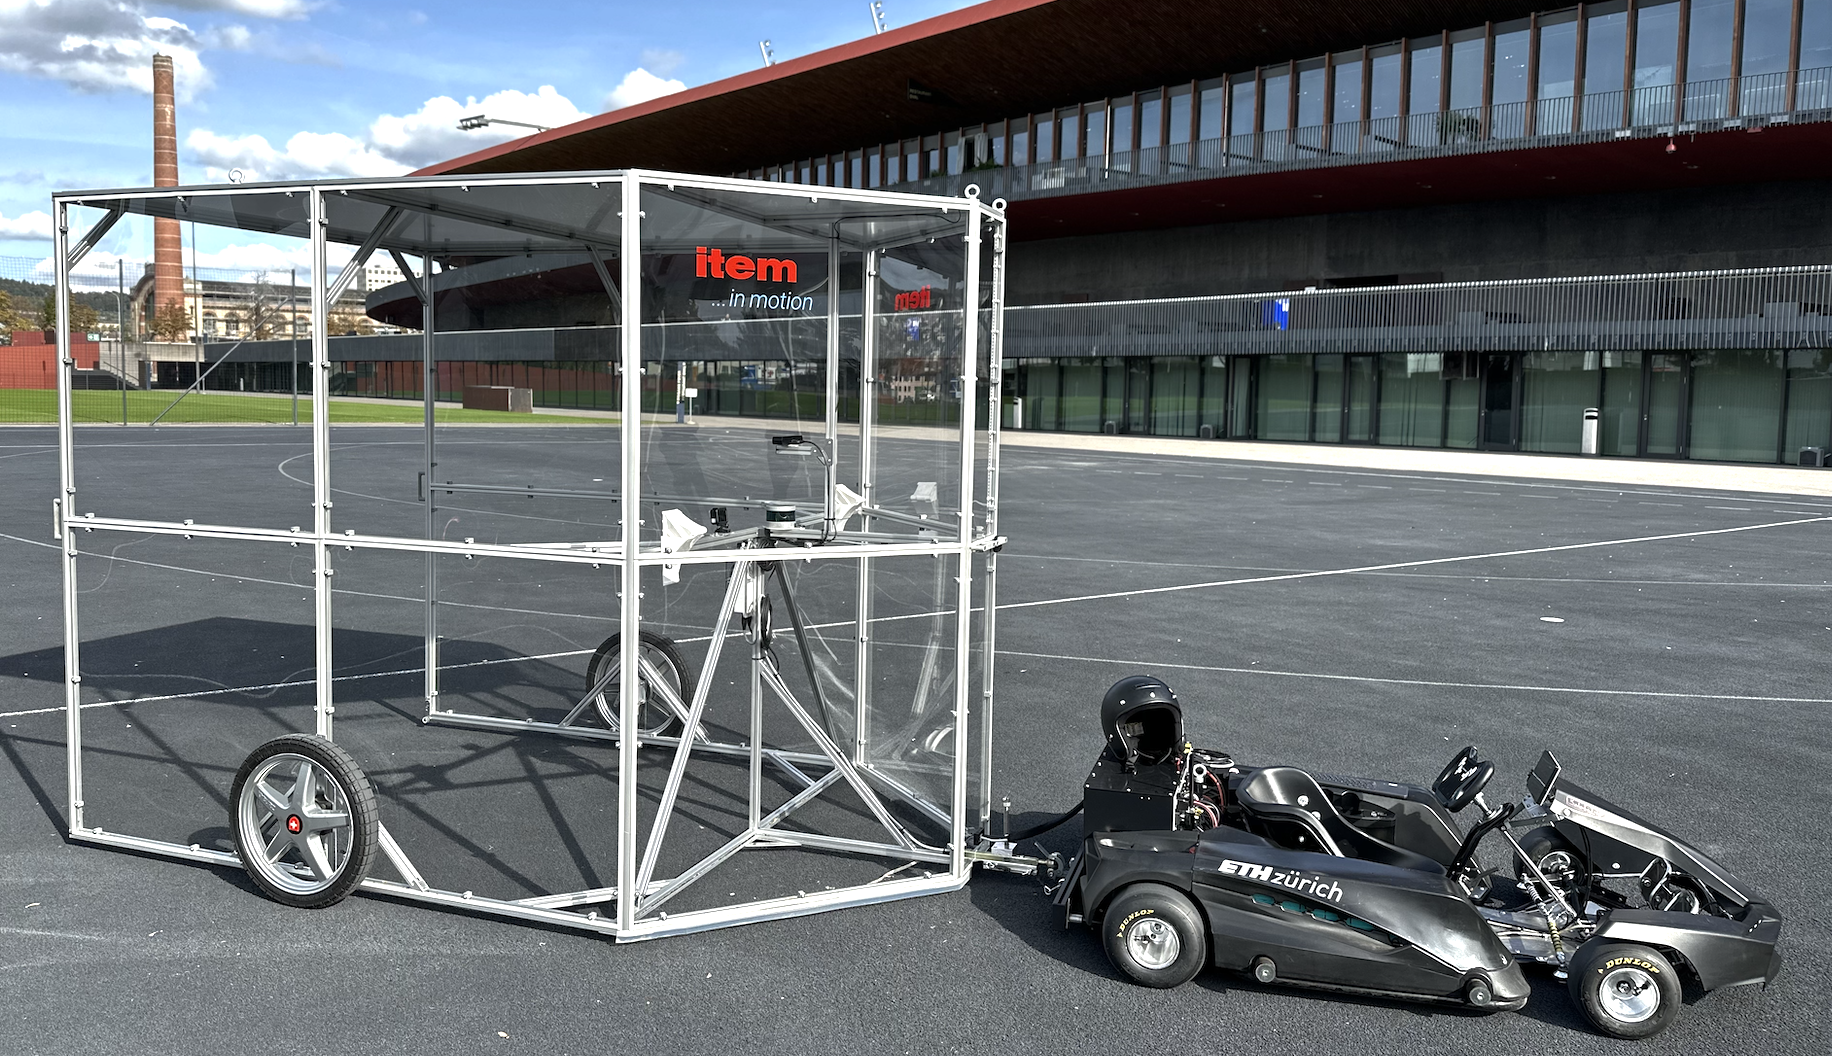
\includegraphics[width=0.47\textwidth]{Windshield} 
	\end{center}
\end{column}
\begin{column}{0.38\textwidth}
\setstretch{0.4}
\onslide <2,3>The usage of an \textbf{autonomous go-kart} improves:
	\begin{itemize}
		\footnotesize
		\item[$\blacktriangleright$] <2->the safety of the maneuver
		\item[$\blacktriangleright$] <2->the reliability and the reusability 
	\end{itemize}
\end{column}
\end{columns}
\vspace{0.7cm}

\onslide <3> \textcolor{emph@Thesis}{\textbf{\small{Contributions}}} \\
\vspace{0.1cm}
\footnotesize
\begin{itemize}
	\setstretch{1.0}
	\footnotesize
	\item[$\blacktriangleright$] <3->Approximated model for the go-kart with the airshield attached
	\item[$\blacktriangleright$] <3->Design a controller to regulate the shield with respect to the runner
	\item[$\blacktriangleright$] <3->Implement and test the controller in simulation and hardware-in-the-loop
\end{itemize}
\end{frame}


%%%%%% MODELING %%%%%%%%%%%%%%%%%%%%%%%%%%%%%%%%%%%%%%%%%%%%%%%%%%%%%%%%%%%%%%%%
\begin{frame}[t]
\frametitle{Modeling of the go-kart with the airshield attached}
\begin{columns}
\begin{column}{0.4\textwidth}
	\begin{center}
  		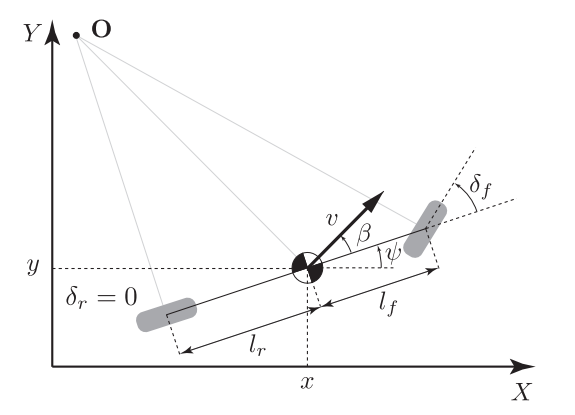
\includegraphics[width=0.75\textwidth]{Bycicle_scheme} 
	\end{center}
\end{column}
\begin{column}{0.6\textwidth}
\onslide <1,2,3,4,5,6,7> \hspace{0.4cm} \textbf{Nonlinear kinematic byclicle model}
	\begin{equation*}
	\begin{cases}
 		\begin{aligned}
			\dot{x}(t) &= v(t) \cos(\psi(t) + \beta(t)) \\
			\dot{y}(t) &= v(t) \sin(\psi(t) + \beta(t)) \\
			\dot{\psi}(t) &= \frac{v(t)}{l_r} \sin(\beta(t)) \\
			\dot{v}(t) &= \frac{F_x(t)}{m} = \frac{1}{m} (C_{m1}a(t) - C_f v(t) - \alert<6>{C_d v^2(t) - C_{roll}}) \\
		\end{aligned}
	\end{cases}
	\end{equation*}
\end{column}
\end{columns}


\begin{columns}
\begin{column}{0.4\textwidth}
\onslide <2,3,4,5,6,7> \begin{block}{}
\centering
\onslide <2,3,4,5,6,7> \begin{itemize}
 	 \footnotesize
	\setstretch{0.8}
	\item[$\blacktriangleright$] High energy-demanding training
	\item[$\blacktriangleright$] Only 50-80 meters executed
\end{itemize}
\end{block}
\end{column}
\begin{column}{0.05\textwidth}
\centering
\onslide <3,4,5,6,7> $\Rightarrow$
\end{column}
\begin{column}{0.35\textwidth}
\onslide <4,5,6,7>\begin{block}{}
\centering
\onslide <4,5,6,7> \begin{itemize}
 	 \footnotesize 
	\setstretch{0.8}
	\item[$\blacktriangleright$] No steeering degree of freedom 
	\item[$\blacktriangleright$] Model can be simplified
\end{itemize}
\end{block}
\end{column}
\end{columns}

\vspace{0.6cm}

\begin{columns}
\hspace{0.8cm}
\begin{column}{0.4\textwidth}
\vspace{-0.9cm}
\onslide <5,6,7>\begin{equation*}
	\begin{cases}
 	\begin{aligned}
		\dot{p}(t) &= v(t) \\
		\dot{v}(t) &= \frac{F(t)}{m} = \frac{1}{m} (C_{m1} a(t) - C_f v(t) \only<7>) \onslide<5,6>{- \alert<6>{C_d v^2(t) - C_{roll}})}
	\end{aligned}
	\end{cases}
\end{equation*}
\end{column}

\begin{column}{0.6\textwidth}
\onslide<7> \hspace{2.5cm}\textbf{Linear time-invariant system}
\onslide<7>\begin{equation*}
    \begin{aligned}
    		\begin{bmatrix}
    			p_{k,t+1} \\
    			v_{k,t+1}
    		\end{bmatrix}
    		& =
    		\begin{bmatrix}
    			1 & dt \\
    			0 & 1-dt\frac{C_f}{m}
    		\end{bmatrix}
    		x_{k,t}
    		+
    		\begin{bmatrix}
    			0 \\
    			dt \frac{C_{m1}}{m}
    		\end{bmatrix}
    		u_t \\
    		& = A \, x_{k,t} + B \, u_t
    \end{aligned}
\end{equation*}
\end{column}
\end{columns}
\begin{columns}
\begin{column}{0.4\textwidth}
\vspace{-0.4cm}
\onslide<6,7> \begin{block}{}
\centering
\onslide<6,7> \begin{itemize}
	\footnotesize
	\item[$\blacktriangleright$] The nonlinear term can be simplified
\end{itemize}
\end{block}
\end{column}
\begin{column}{0.49\textwidth}
\end{column}
\end{columns}
\end{frame}


%%%%%% APPLICATION SET-UP %%%%%%%%%%%%%%%%%%%%%%%%%%%%%%%%%%%%%%%%%%%%%%%%%%%%%%%%%%%%
\begin{frame}[t]
\frametitle{Application setup}

\vspace{-0.2cm}
\onslide<1,2,3,4,5,6,7>\begin{columns}
\begin{column}{0.67\textwidth}
Aerodynamics studies $^1$ have shown that, by running in the slipstream of a shield:
\begin{itemize}
	\footnotesize
	\item[$\blacktriangleright$] Runner is isolated from the drag resistance
	\item[$\blacktriangleright$] A pushing force from behind enhances the speed
\end{itemize}
\vspace{0.3cm}
\onslide<1,2,3,4,5,6,7>Reference distance: $d_\text{des} = 2.5$ meters
\vspace{0.3cm}


{\color{gray} \scriptsize 
$^1$ Italian National Olympic Committee (CONI) Institute of Sports Science \\
\hspace{0.2cm} “Aerodynamic Shield – new training support technologies”}
\end{column}
\begin{column}{0.32\textwidth}
	\begin{center}
  		\hspace{-0.9cm}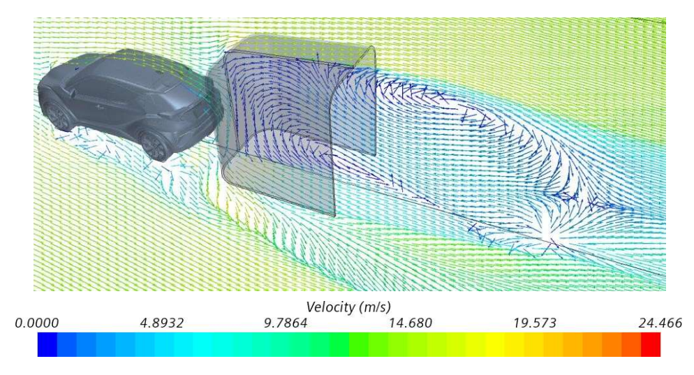
\includegraphics[width=1.2\textwidth]{Aerodynamics} 
	\end{center}
\end{column}
\end{columns}

\vspace{-0.2cm}
\begin{columns}
\begin{column}{0.15\textwidth}
\onslide<2,3,4,5,6,7>\begin{block}{}
\centering
\textbf{\small{Controller \\ objectives}}
\end{block}
\end{column}
\begin{column}{0.82\textwidth}
\onslide<3,4,5,6,7>\begin{block}{}
\begin{itemize}
	\footnotesize
	\item[$\blacktriangleright$]<3-> Maintain the desired reference distance between airshield and runner
	\item[$\blacktriangleright$]<4-> Match, as closely as possible, kart velocity with the runner's one
\end{itemize}
\end{block}
\end{column}
\end{columns}

\vspace{-0.2cm}
\begin{columns}
\begin{column}{0.15\textwidth}
\onslide<5,6,7>\begin{block}{}
\centering
\textbf{\small{Controllers \\ formulations}}
\end{block}
\end{column}
\begin{column}{0.22\textwidth}
\onslide<5,6,7>\begin{block}{}
\centering
\textcolor{emph@Thesis}{\textbf{Gain Scheduling \\ Linear Quadratic Regulator}}
\end{block}
\end{column}
\hspace{-0.4cm}
\begin{column}{0.3\textwidth}
\onslide<5,6,7>\begin{block}{}
\centering
\textcolor{mygreen}{\textbf{Linear Model Predictive Controller}}
\end{block}
\end{column}
\hspace{-0.4cm}
\begin{column}{0.23\textwidth}
\onslide<5,6,7>\begin{block}{}
\centering
\textcolor{red}{\textbf{Offset-free \\ Model Predictive Controller}}
\end{block}
\end{column}
\end{columns}

\vspace{0.1cm}
\begin{columns}
\onslide<6,7>\begin{column}{0.3\textwidth}
	\begin{center}
  		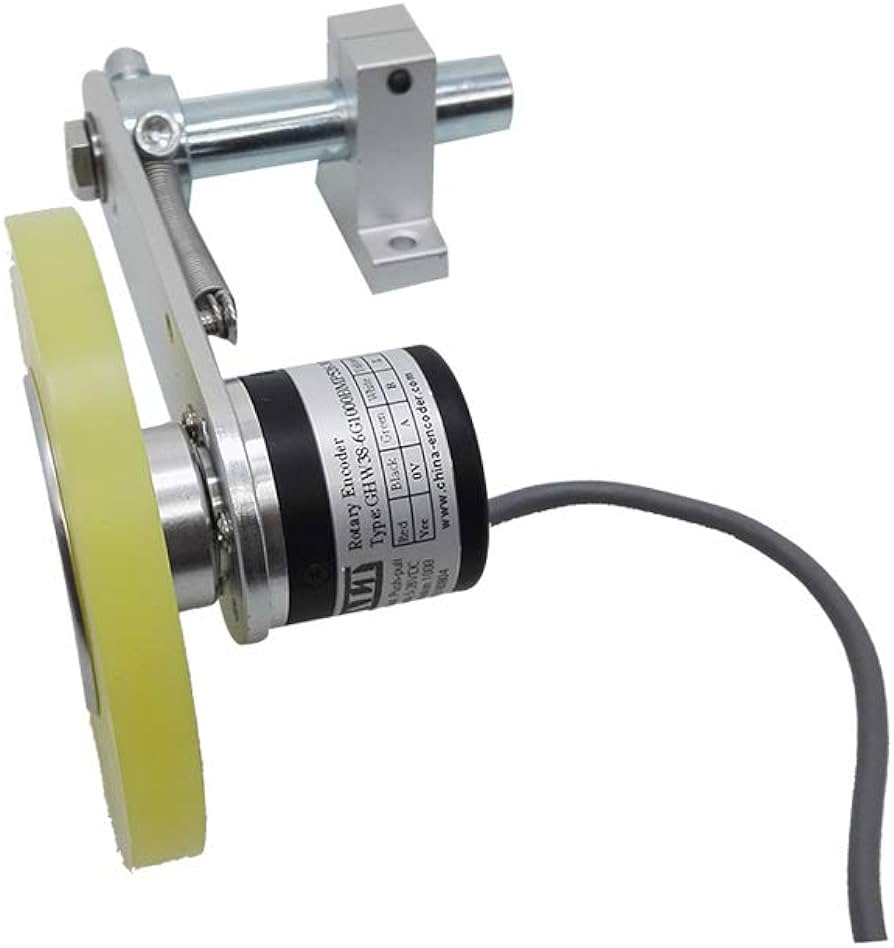
\includegraphics[width=0.23\textwidth]{Wheel_Encoder} 
	\end{center}
\centering
\textbf{Wheel Encoders} \\
Absolute kart velocity $v_k$
\end{column}

\onslide<6,7>\begin{column}{0.3\textwidth}
	\begin{center}
  		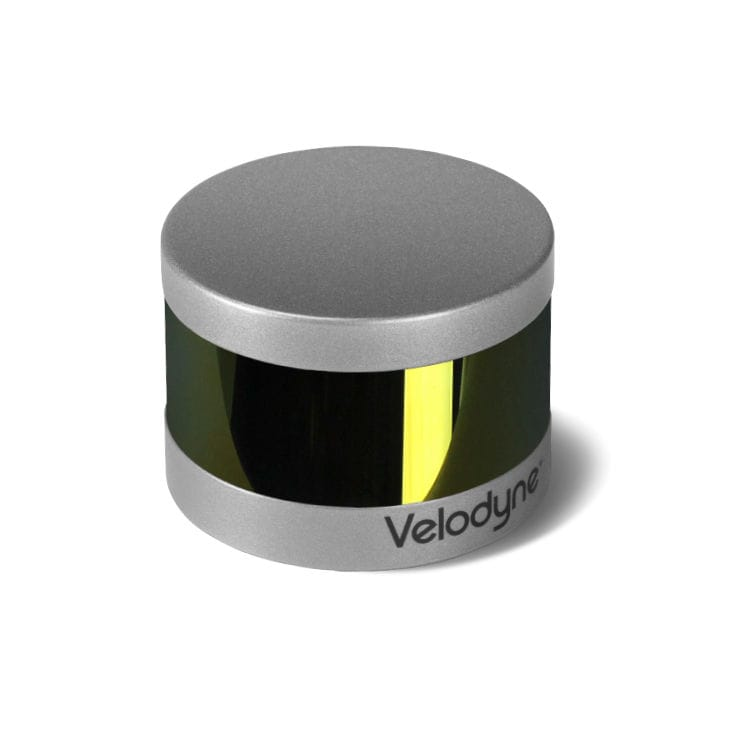
\includegraphics[width=0.23\textwidth]{Lidar} 
	\end{center}
\centering
\textbf{LiDAR (Velodyne)} \\
Relative distance $\Delta p = p_k - p_r$
\end{column}

\onslide<7>\begin{column}{0.4\textwidth}
\hspace{1.5cm} \textbf{Estimated}:
\begin{itemize}
	\footnotesize
	\item[$\blacktriangleright$] Relative velocity  $\Delta v = v_k - v_r$
	\item[$\blacktriangleright$] Absolute runner acceleration  $a_r$
\end{itemize}
\end{column}
\end{columns}
\end{frame}



%%%%%% LQR %%%%%%%%%%%%%%%%%%%%%%%%%%%%%%%%%%%%%%%%%%%%%%%%%%%%%%%%%%%%%%%%%%%%
\begin{frame}
\frametitle{Gain Scheduling Linear Quadratic Regulator}
\centering
\textcolor{emph@Thesis}{\textbf{\small{Linear Quadratic Regulator}}} 
\vspace{0.2cm}
\begin{columns}
\begin{column}{0.4\textwidth}
\centering

\begin{columns}
\onslide <1,2,3,4>\begin{column}{0.6\textwidth}
\centering
\begin{block}{}
\begin{equation*}
    h_t =
    \begin{bmatrix}
        \Delta p_t  \\
        \Delta v_t
    \end{bmatrix}
	=
    \begin{bmatrix}
        p_{k,t} - p_{r,t} \\
        v_{k,t} - v_{r,t}
    \end{bmatrix}
\end{equation*}

\end{block}
\end{column}

\begin{column}{0.3\textwidth}
\centering
\begin{block}{}
\begin{equation*}
    h_{\text{des}} =
    \begin{bmatrix}
        d_{\text{des}} \\
        0
    \end{bmatrix}
\end{equation*}
\end{block}
\end{column}
\end{columns}

\end{column}

\onslide<1,2,3,4>\begin{column}{0.6\textwidth}
\centering
\begin{itemize}
	\footnotesize
	\item[$\blacktriangleright$] Offline: Compute the Linear Quadratic Regulator: $K$
	\item[$\blacktriangleright$] Control the system using the feedback $u^* = - K (h_t - h_{\text{des}}) $
\end{itemize}
\end{column}
\end{columns}

\vspace{1.0cm}
\centering
\onslide<2,3,4>\textcolor{emph@Thesis}{\textbf{\small{Gain Scheduling Approach}}} 

\begin{columns}
\begin{column}{0.5\textwidth}
\vspace{0.2cm}
\onslide<2,3,4>\begin{block}{}
\centering
\textbf{Catch-up maneuver $K_\text{catch}$} \\
\end{block}
\onslide<3,4>In the first couple of seconds the runner has an acceleration exceeding the maximum go-kart capabilities.
\onslide<3,4>\begin{itemize}
\vspace{0.1cm}
\footnotesize
	\item[$\blacktriangleright$] Ask the runner to start the sprint at $\Delta p_\text{init} = d_\text{des} + \bar{d}$
	\item[$\blacktriangleright$] Control using $u^* = - K_\text{catch} (h_t - h_{\text{des}}) $
	\item[$\blacktriangleright$] Match the velocities with a safe distance bigger than $d_\text{des}$
\end{itemize}

\end{column}
\begin{column}{0.5\textwidth}
\vspace{-0.1cm}
\onslide<2,3,4>\begin{block}{}
\centering
\textbf{Cruise control maneuver $K_\text{cruise}$} \\
\end{block}
\onslide<4>Once the runner and go-kart velocities are matched at 80\%
\onslide<4>\begin{itemize}
\vspace{0.1cm}
\footnotesize
	\item[$\blacktriangleright$] Control using $u^* = - K_\text{cruise} (h_t - h_{\text{des}}) $
	\item[$\blacktriangleright$] Reduce the distance up to the reference $d_\text{des}$
	\item[$\blacktriangleright$] Maintain the steady state condition
\end {itemize}
\end{column}
\end{columns}

\end{frame}

%%%%%% LQR 2 %%%%%%%%%%%%%%%%%%%%%%%%%%%%%%%%%%%%%%%%%%%%%%%%%%%%%%%%%%%%%%%%%%
\begin{frame}
\frametitle{Gain Scheduling Linear Quadratic Regulator}
\begin{center}
  	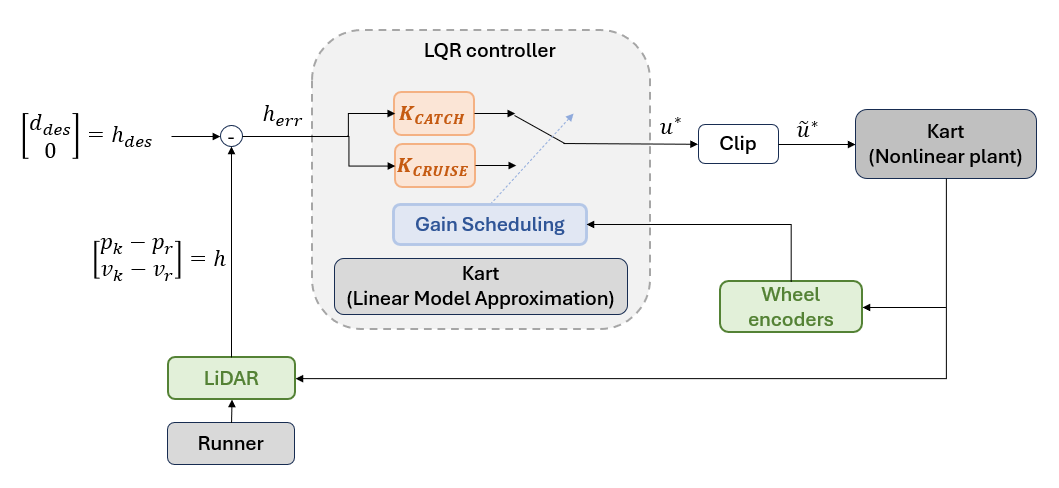
\includegraphics[width=0.6\textwidth]{LQR_scheme} 
\end{center}
\vspace{-0.1cm}
\begin{columns}

\onslide<1,2,3,4,5,6>\begin{column}{0.4\textwidth}
\begin{block}{}
\centering
\textcolor{emph@Thesis}{\textbf{Gain Scheduling}} 
\begingroup
\setlength{\jot}{0.4ex}
\begin{equation*}
\begin{aligned}
	&\textbf{if} \,\, (v_{k,t} \geq 0.8 \, v_{r,t}) \,\, \textbf{and} \,\, (\text{catched = false}): \\
	& \quad \text{catched = true;} \\
	&\textbf{end if} \\
	&\textbf{if} \,\, \text{(catched = false):} \\
	& \quad u^* = - K_{\text{catch}} (h_t - h_{\text{des}}) ; \\
	&\textbf{else} \\
	& \quad u^* = - K_{\text{cruise}} (h_t - h_{\text{des}}); \\
	&\textbf{end if}
\end{aligned}
\end{equation*}
\endgroup
\end{block}
\end{column}

\begin{column}{0.40\textwidth}
\onslide<2,3,4,5,6>\begin{block}{}
\centering
\textcolor{mygreen}{\textbf{Pros of LQR controller}}
\begin{itemize}
\footnotesize
	\item[$\blacktriangleright$]<2-> Reduced computational effort
\end{itemize}
\end{block}
\vspace{-0.2cm}
\onslide<3,4,5,6>\begin{block}{}
\centering
\textcolor{red}{\textbf{Cons of LQR controller}} \\
\begin{itemize}
\footnotesize
	\item[$\blacktriangleright$]<3-> No explicit constraints management
	\item[$\blacktriangleright$]<4-> Actuator limits: $a_\text{min} \leq u \leq a_\text{max}$
	\item[$\blacktriangleright$]<5-> No state constraints (i.e. $\Delta p \leq d_\text{safe}$)
	\item[$\blacktriangleright$]<6-> No assumption on runner expected behaviour
\end{itemize}
\end{block}
\end{column}

\end{columns}
\end{frame}

%%%%%% MPC %%%%%%%%%%%%%%%%%%%%%%%%%%%%%%%%%%%%%%%%%%%%%%%%%%%%%%%%%%%%%%%%%%%
\begin{frame}
\frametitle{Linear Model Predictive Control}
\begin{columns}
\begin{column}{0.6\textwidth}
\onslide<1,2,3,4,5,6>\begin{equation*}
\begin{aligned}
        \begin{bmatrix}
            \Delta p_{t+1}  \\
            \Delta v_{t+1} \\
            v_{k,t+1}
        \end{bmatrix}
        & =
        \begin{bmatrix}
            1 & dt & 0 \\
            0 & 1 & -dt\frac{C_f}{m} \\
            0 & 0 & 1-dt\frac{C_f}{m}
        \end{bmatrix}
        x_{p,t}
        +
        \begin{bmatrix}
            0 \\
            dt \frac{C_{m1}}{m} \\
            dt \frac{C_{m1}}{m}
        \end{bmatrix}
        u_t + 
	 \alert<2>{
        \begin{bmatrix}
        0 \\
        - dt a_{r,t} \\
        0
        \end{bmatrix} }\\
        & = A_p \, x_{p,t} + B_p \, u_t \alert<2>{+ a_t}
\end{aligned}
\end{equation*}
\end{column}

\begin{column}{0.43\textwidth}
\onslide<2,3,4,5,6>\begin{block}{}
\centering
\textcolor{mygreen}{\textbf{Pros of MPC controller}} 
\begin{itemize}
	\footnotesize
	\item[$\blacktriangleright$] <2->Incorporate a runner model in the predictions
	\item[$\blacktriangleright$] <3-> Semplification of the control architecture
	\item[$\blacktriangleright$] <4-> Constraints explicitly included in the formulation
	\item[$\blacktriangleright$] <5-> Safety guarantees via state constraints

\end{itemize}
\end{block}
\end{column}

\end{columns}

\vspace{0.1cm}
\begin{columns}
\begin{column}{0.55\textwidth}
	\begin{center}
  		\onslide<3,4,5,6>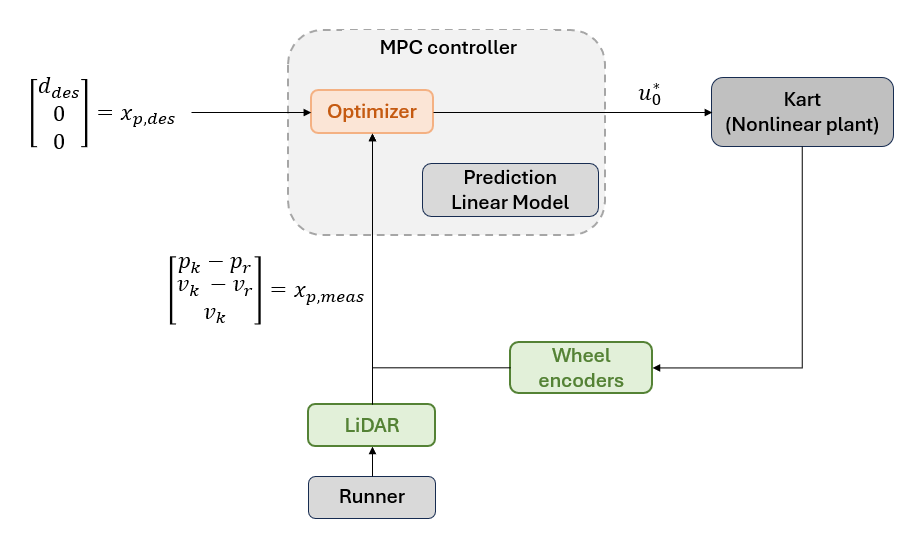
\includegraphics[width=1\textwidth]{MPC_scheme} 
	\end{center}
\end{column}

\begin{column}{0.40\textwidth}
\onslide<4,5,6>\begin{block}{}
\centering
\textcolor{orange}{\textbf{Optimizer}} 
\begin{equation*}
\begin{alignedat}{2}
	\min_{\substack{\boldsymbol{x}, \boldsymbol{u}}}\quad &\sum_{i=t}^{t+N-1} \|(x_{p,i|t} - x_{p,\text{des}})\|_Q \, +  \|u_{i|t}\|_R &&   \\
	\text{subj. to} & \quad x_{p,i+1|t}  = A_p \, x_{p,i|t} + B_p \, u_{i|t} + a_t  && \\
    &\alert<4>{\quad a_{\text{min}} \leq u_{i|t} \leq a_{\text{max}}} && \\
    &\alert<5>{\quad d_{\text{safe}}\leq \Delta p_{i|t}} &&  \\
    &\quad x_{p,t|t} = x_{p,\text{meas}} &&
\end{alignedat}
\end{equation*}
\end{block}
\onslide<6>\begin{block}{}
\centering
\textcolor{red}{\textbf{Cons of MPC controller}}
\begin{itemize}
\footnotesize
	\item[$\blacktriangleright$] Higher computational effort
\end{itemize}
\end{block}
\end{column}
\end{columns}
\end{frame}


%%%%%% OFFSET-FREE MPC %%%%%%%%%%%%%%%%%%%%%%%%%%%%%%%%%%%%%%%%%%%%%%%%%%%%%%%%%%%%%
\begin{frame}
\frametitle{Offset-free Model Predictive Control $^1$}
\begin{columns}
\begin{column}{0.55\textwidth}
\onslide<1,2,3,4,5>\begin{block}{}
\centering
\textcolor{red}{\textbf{Cons of MPC controller}} 
\begin{itemize}
\footnotesize
	\item[$\blacktriangleright$]  A nonlinear system is controlled using a linear prediction model
	\item[$\blacktriangleright$] \textbf{Model-plant mismatch} can lead to suboptimal performances
\end{itemize}
\end{block}
\end{column}
\hspace{-0.2cm}
\begin{column}{0.02\textwidth}
\centering
\vspace{0.1cm}
\onslide<2,3,4,5>$\Rightarrow$
\end{column}
\hspace{-0.2cm}
\begin{column}{0.46\textwidth}
\onslide<2,3,4,5>\begin{block}{}
\centering
\textcolor{mygreen}{\textbf{Pros of Offset-free MPC controller}} 
\begin{itemize}
\footnotesize
	\item[$\blacktriangleright$] Estimate the non linearity via Luemberger observer
	\item[$\blacktriangleright$] Modify the MPC formulation to achieve offset-free
\end{itemize}
\end{block}
\end{column}
\end{columns}

\begin{columns}
\begin{column}{0.6\textwidth}
	\begin{center}
  		\onslide<3,4,5>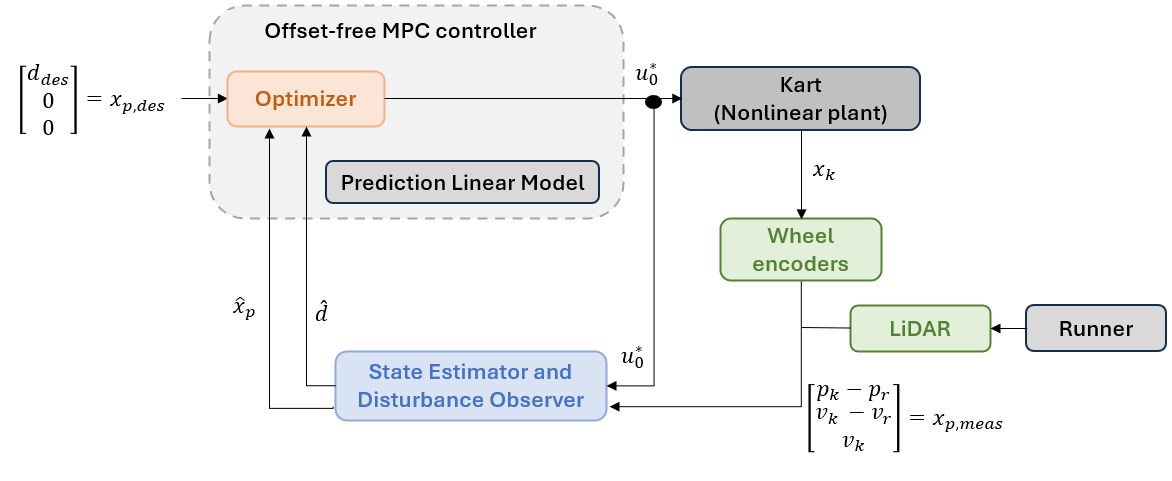
\includegraphics[width=1.05\textwidth]{MPC_ofhard_scheme} 
	\end{center}
\end{column}
\hspace{0.2cm}
\begin{column}{0.43\textwidth}
\onslide<4,5>\begin{block}{}
\centering
\textcolor{orange}{\textbf{Optimizer}} 
\begin{equation*}
\scriptsize
\begin{alignedat}{2}
	\min_{\substack{\boldsymbol{x}, \boldsymbol{u}}}\quad & \sum_{i=t}^{t+N-1} \| x_{p,i|t} - \bar{x}_t \|_Q +  \| u_{i|t} - \bar{u}_t\|_R &&  \\
	\text{subj. to} & \quad x_{p,i+1|t}  = A_p \, x_{p,i|t} + B_p \, u_{i|t} + a_t + B_d \, d_{i|t} &&  \\
    & \quad d_{i+1|t}  = d_{i|t} && \\
    &\quad a_{\text{min}} \leq u_{i|t} \leq a_{\text{max}}&& \\
    &\quad d_{\text{safe}}\leq \Delta p_{i|t} &&  \\
    &\quad x_{p,t|t} = \hat{x}_t && \\
    &\quad d_{t|t} = \hat{d}_t && 
\end{alignedat}
\end{equation*}
\end{block}
\end{column}
\end{columns}

\vspace{0.1cm}
\begin{columns}

\onslide<5>\begin{column}{0.7\textwidth}
\begin{block}{}
\centering
\textcolor{emph@Thesis}{\textbf{Disturbance Observer}} 
\begin{equation*}
\scriptsize
    	\begin{bmatrix}
    	 \hat{x}_{p,t+1} \\
            \hat{d}_{t+1}
        \end{bmatrix}
        = 
    	\begin{bmatrix}
    		A_p & B_d \\
    		0 & I
    	\end{bmatrix}
    	\begin{bmatrix}
    		\hat{x}_{p,t} \\
    		\hat{d}_t
    	\end{bmatrix}
        +
    	\begin{bmatrix}
    		B_p \\
    		0
    	\end{bmatrix}
        u +
        \begin{bmatrix}
            L_x \\
            L_d \\
        \end{bmatrix} 
        ( - y_{m,t} +
        \begin{bmatrix}
            C & C_d 
        \end{bmatrix}
        \begin{bmatrix}
            \hat{x}_{p,t} \\
            \hat{d}_t
        \end{bmatrix} ) 
\end{equation*}
\end{block}
\end{column}

\begin{column}{0.3\textwidth}

\vspace{1cm}

\onslide<1,2,3,4,5> \color{gray} \scriptsize $^1$ U. Maeder, F. Borrelli, M. Morari \\ 
“Linear offset-free Model Predictive Control”
\end{column}
\end{columns}

\end{frame}

%%%%%% SIMULATION TESTS %%%%%%%%%%%%%%%%%%%%%%%%%%%%%%%%%%%%%%%%%%%%%%%%%%%%%%%%%%%%
\begin{frame}
\frametitle{Simulation tests and Controllers comparison}
\begin{columns}
\begin{column}{0.57\textwidth}
\centering
\onslide<1,2,3>\begin{block}{}
\begin{itemize}
\footnotesize
	\setstretch{0.8}
	\item[$\blacktriangleright$] Simulation implementation of the three controllers
	\item[$\blacktriangleright$] Tests on the same velocity profile (professional athlete)
\end{itemize}
\end{block}
\vspace{-0.2cm}
	\begin{center}
  		\onslide<1,2,3>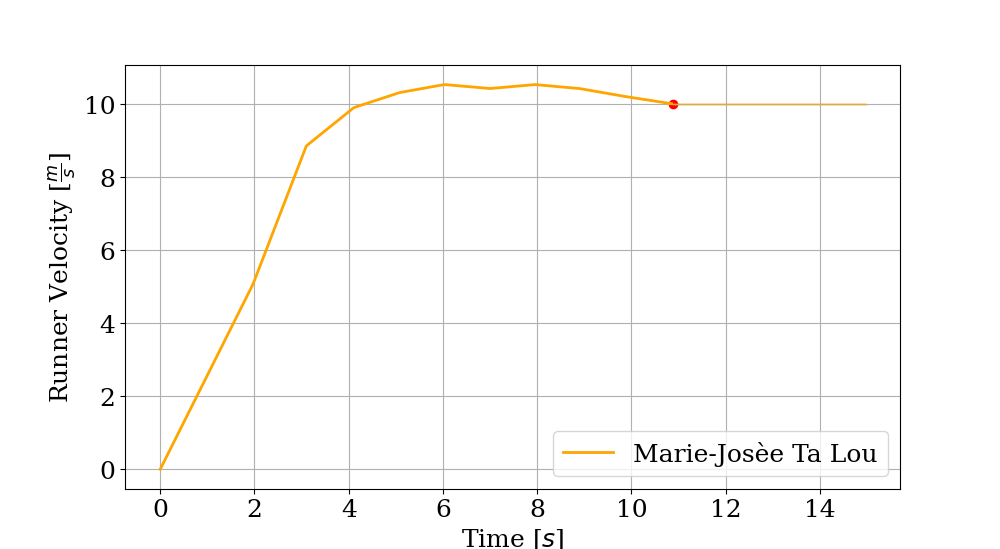
\includegraphics[width=0.6\textwidth]{Test_Velocities} 
	\end{center}
\onslide<2,3>\textbf{Initial distance:}
\centering
\onslide<2,3>$\Delta p_\text{init} = d_\text{des} + \bar{d}, \quad \bar{d}= 4$m
	\begin{center}
  		\onslide<3>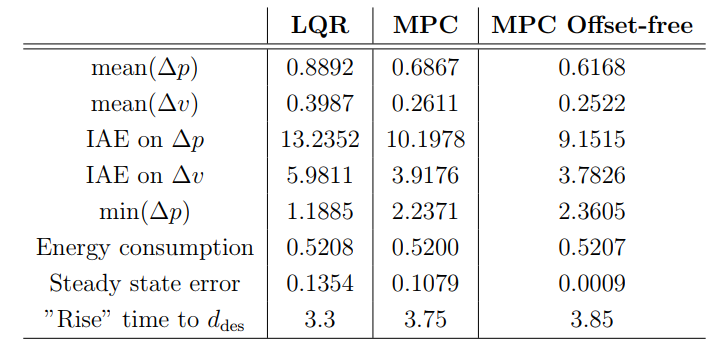
\includegraphics[width=0.7\textwidth]{Ta_Lou/Table} 
	\end{center}


\end{column}
\onslide<3>\begin{column}{0.43\textwidth}
	\begin{center}
  		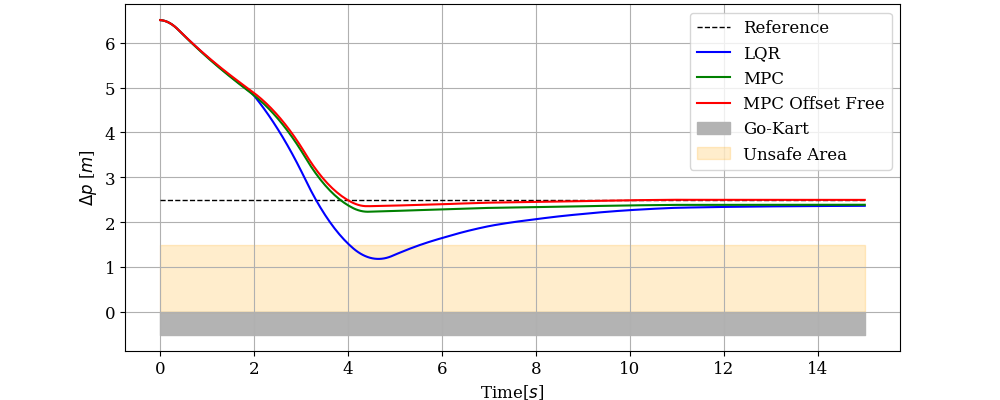
\includegraphics[width=1\textwidth]{Ta_Lou/Deltap} 
	\end{center}
	\vspace{-0.4cm}
	\begin{center}
  		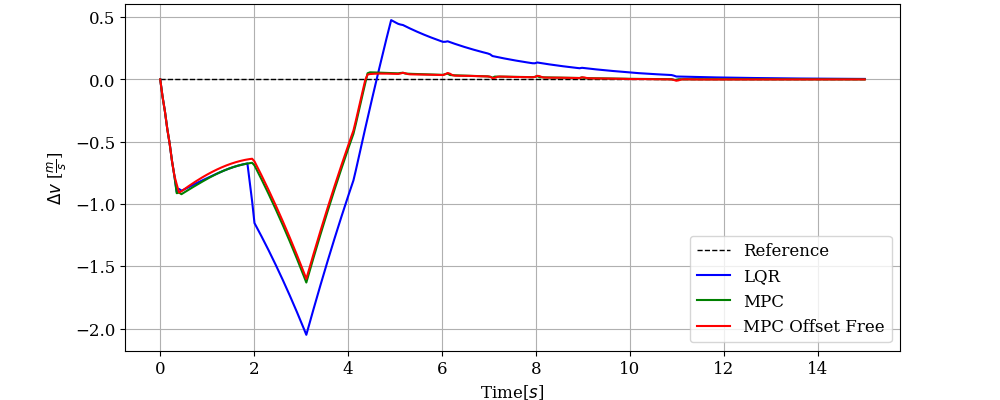
\includegraphics[width=1\textwidth]{Ta_Lou/Deltav} 
	\end{center}
	\vspace{-0.4cm}
	\begin{center}
  		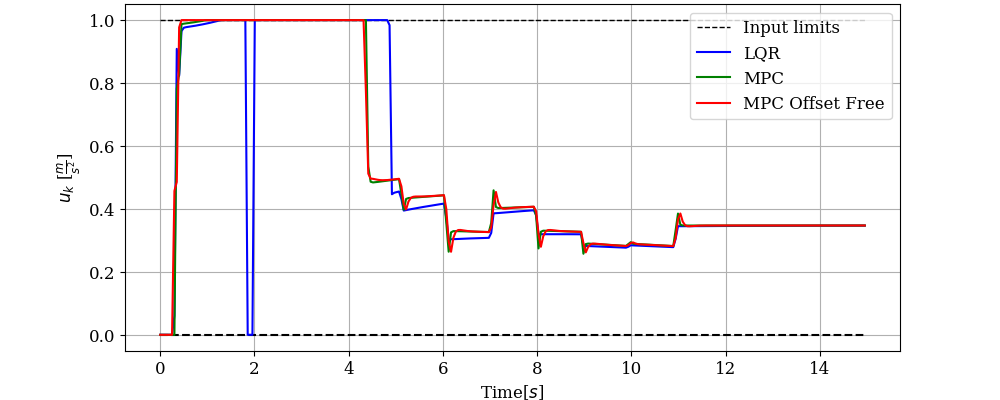
\includegraphics[width=1\textwidth]{Ta_Lou/Input} 
	\end{center}
\end{column}
\end{columns}
\end{frame}


%%%%%% HARDWARE TESTS CATCH-UP %%%%%%%%%%%%%%%%%%%%%%%%%%%%%%%%%%%%%%%%%%%%%%%%%%%%%%

\begin{frame}
\frametitle{Hardware-in-the-loop tests}
\centering
Focus on the catch-up maneuver
\begin{center}
\href{video.mp4}{
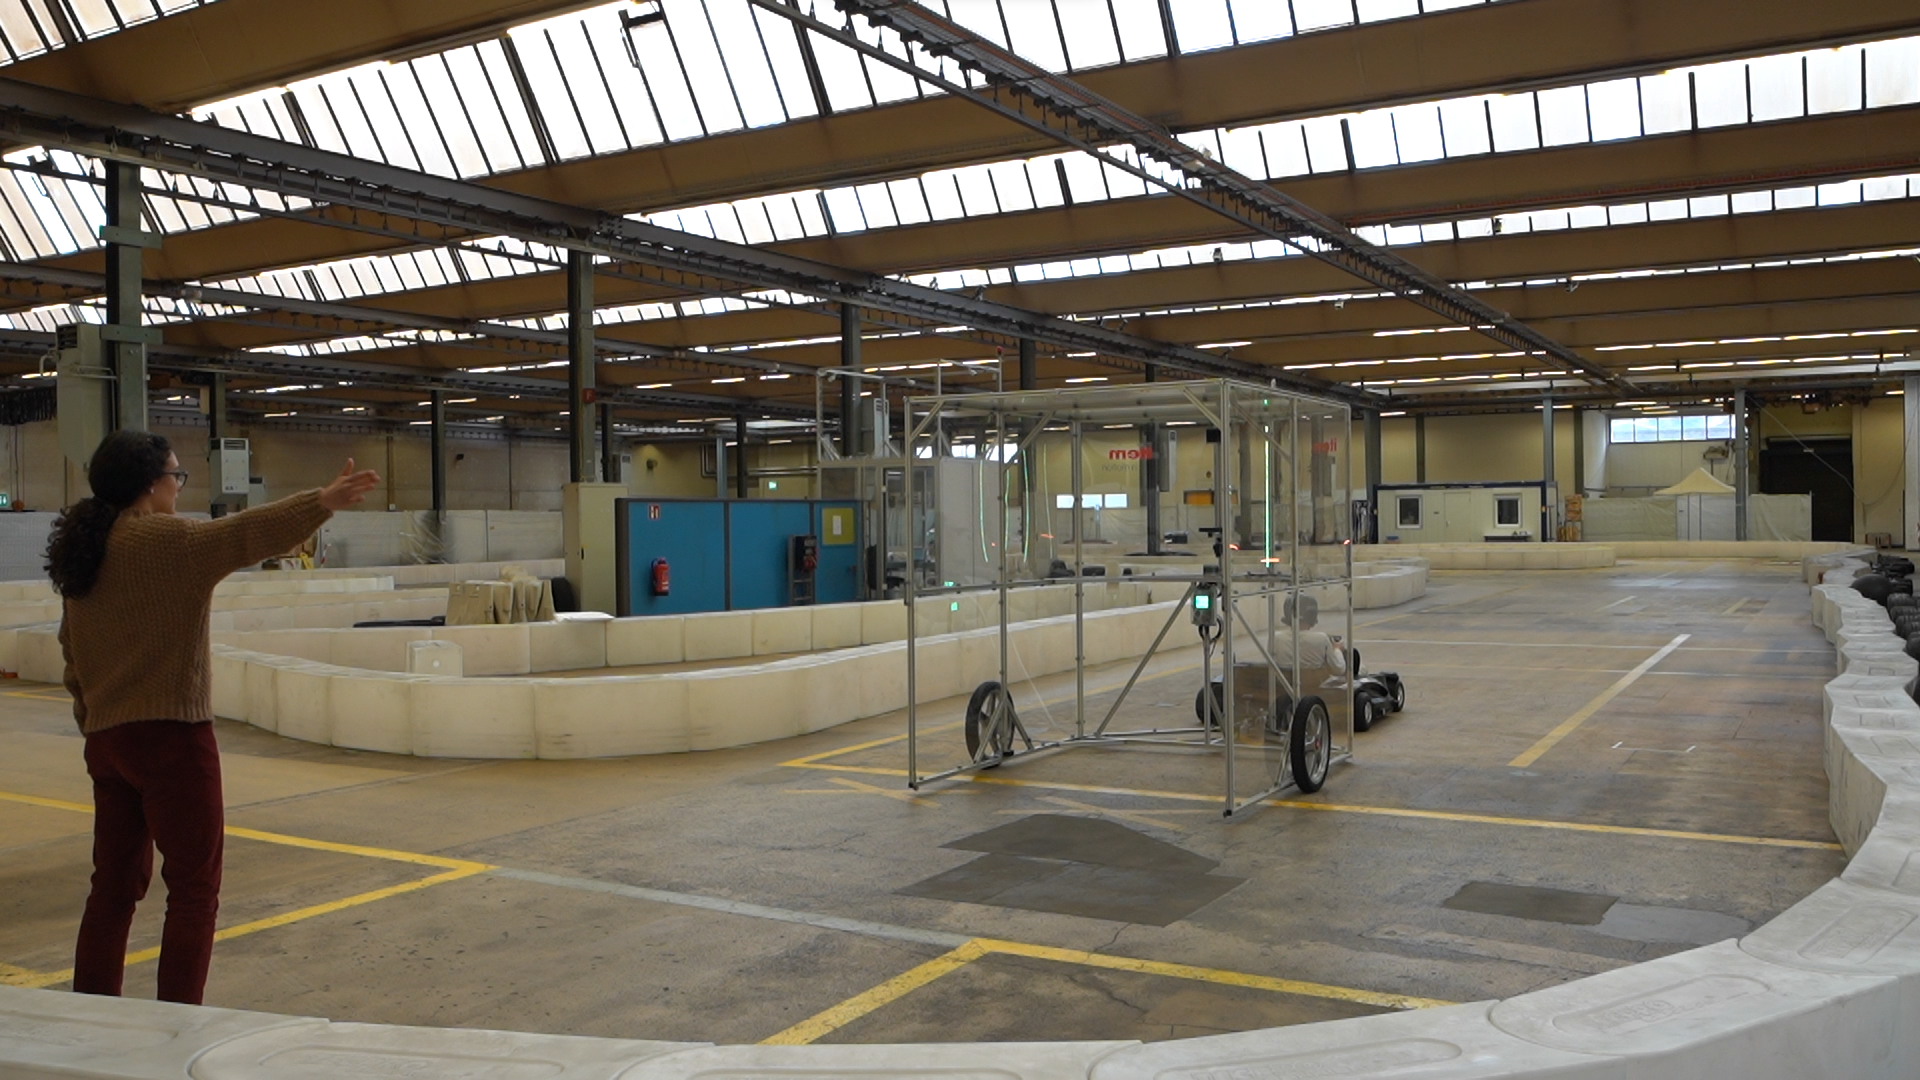
\includegraphics[scale=0.25]
{Poster2}}
\end{center}
\end{frame}

%%%%%% HARDWARE TESTS STEADY-STATE %%%%%%%%%%%%%%%%%%%%%%%%%%%%%%%%%%%%%%%%%%%%%%%%%%%
\begin{frame}
\frametitle{Hardware-in-the-loop tests}
\centering
Focus on maintaining a constant distance with the runner having an almost constant velocity
\begin{center}
\href{Double.mp4}{
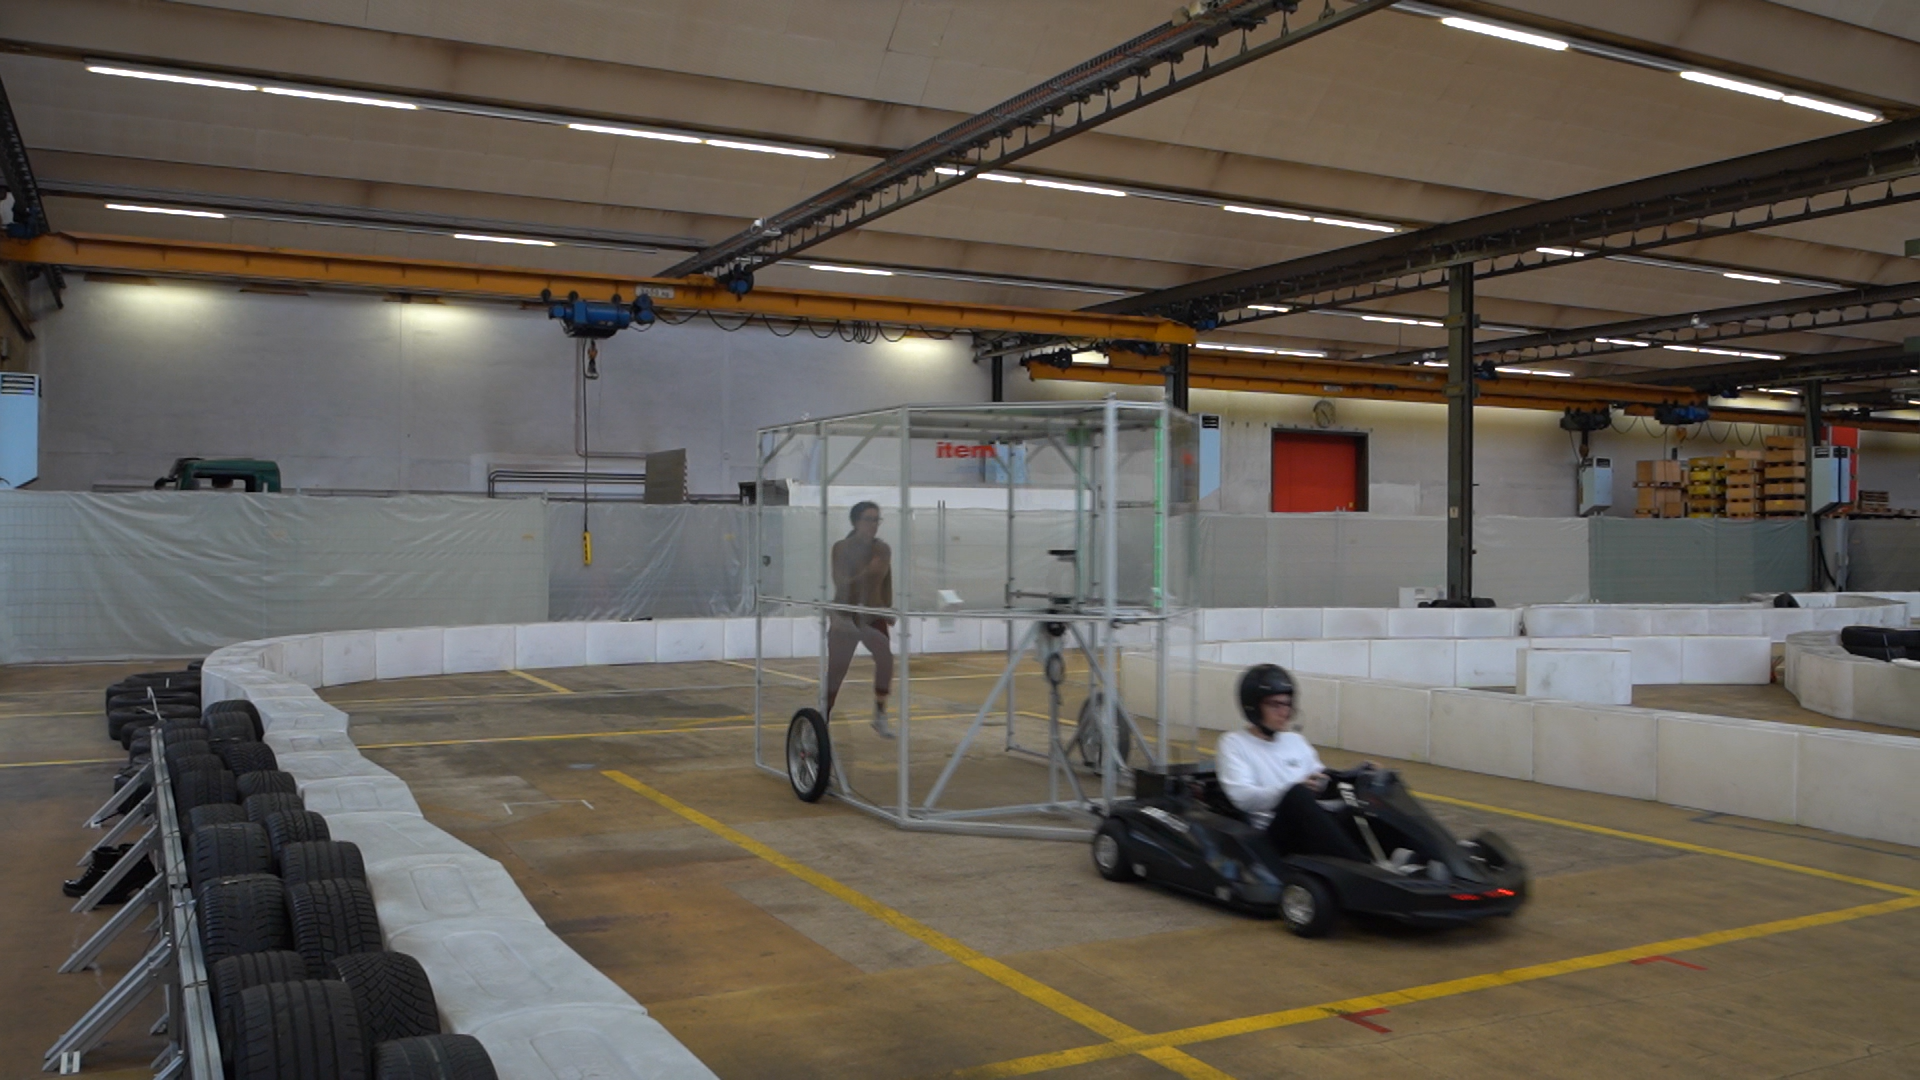
\includegraphics[scale=0.25]
{Poster}}
\end{center}

\end{frame}




%%%%%% CONCLUSIONS %%%%%%%%%%%%%%%%%%%%%%%%%%%%%%%%%%%%%%%%%%%%%%%%%%%%%%%%%%%%%%
\begin{frame}
\frametitle{Conclusion}
%\vspace{0.3cm}
\begin{columns}
\begin{column}{0.55\textwidth}
\onslide<1,2,3>\textcolor{emph@Thesis}{\textbf{\small{Contributions}}} 
\vspace{0.2cm}
\onslide<1,2,3>\begin{itemize}
	\footnotesize
	\item[$\blacktriangleright$] Analysis of the application and requirements definition
	\item[$\blacktriangleright$] Control design
	\begin{itemize}
		 \setlength{\itemsep}{4pt}
		\item[$\triangleright$] Gain Scheduling Linear Quadratic Regulator
		\item[$\triangleright$] Linear Model Predictive Control
		\item[$\triangleright$] Offset-free Model Predictive Control
	\end{itemize}
	\item[$\blacktriangleright$] Simulation test and numerical comparison of performances
	\item[$\blacktriangleright$] Hardware-in-the-loop implementation and tests
\end{itemize}
\end{column}

\vspace{0.3cm}
\begin{column}{0.4\textwidth}
	\begin{center}
  		\onslide<1,2,3>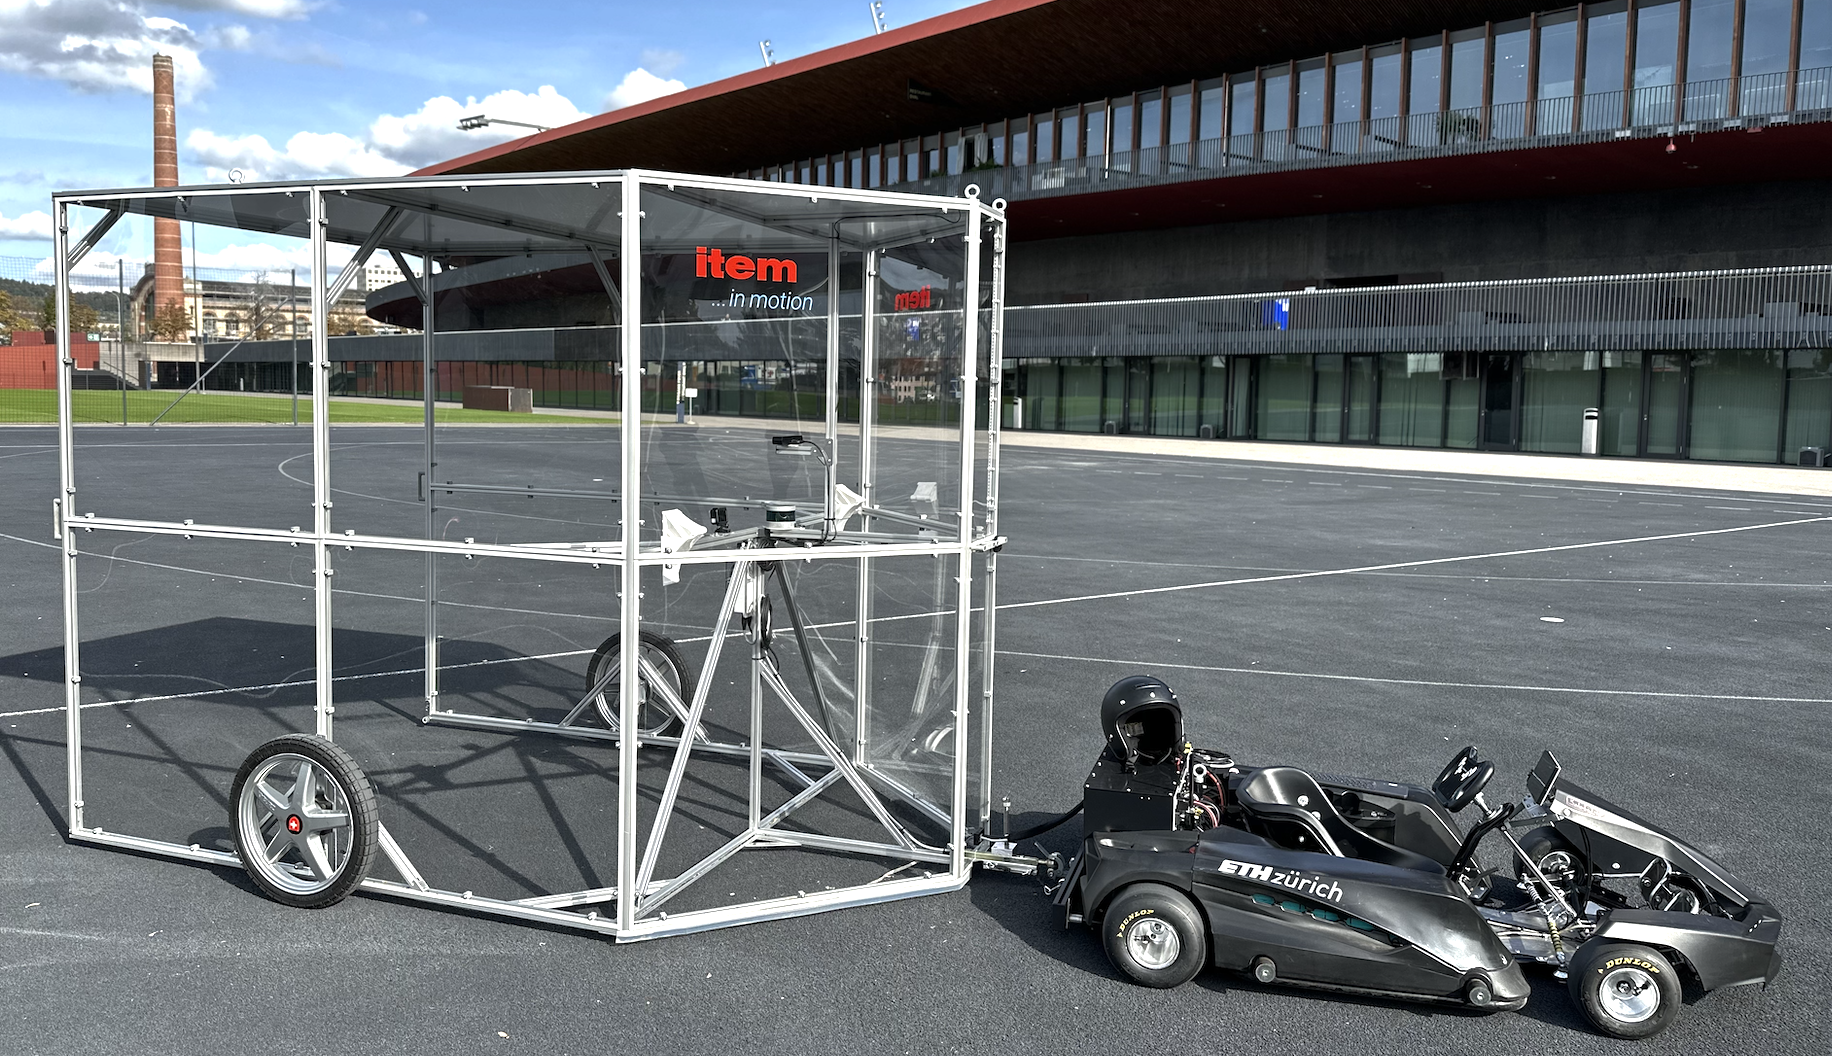
\includegraphics[width=1\textwidth]{Windshield} 
	\end{center}

\begin{columns}
\begin{column}{0.2\textwidth}
	\begin{center}
  		\onslide<1,2,3>
\includegraphics[width=1\textwidth]{ROS2}
	\end{center}
\end{column}
\hspace{-0.6cm}
\begin{column}{0.2\textwidth}
	\begin{center}
  		\onslide<1,2,3>
\includegraphics[width=0.8\textwidth]{Docker} 
	\end{center}
\end{column}
\hspace{-0.6cm}
\begin{column}{0.2\textwidth}
	\begin{center}
  		\onslide<1,2,3>
\includegraphics[width=0.7\textwidth]{Python}
	\end{center}
\end{column}
\hspace{-0.6cm}
\begin{column}{0.2\textwidth}
	\begin{center}
  		\onslide<1,2,3>
\includegraphics[width=0.9\textwidth]{GitHub} 
	\end{center}
\end{column}
\end{columns}

\end{column}
\end{columns}

\onslide<2,3>\textcolor{emph@Thesis}{\textbf{\small{Future developments}}} 
\vspace{0.2cm}
\onslide<2,3>\begin{itemize}
	\footnotesize
	\item[$\blacktriangleright$] Robust MPC formulation using the estimated disturbance
	\item[$\blacktriangleright$] Learning MPC formulation for enhance the runner future behaviour prediction	
	\item[$\blacktriangleright$] Improve the runner acceleration estimation
\end{itemize}

\onslide<3>\vspace{0.8cm} \hspace{5cm} \textcolor{purple}{\textbf{\small{Thanks for your attention}}} 
\end{frame}

\begin{frame}
\end{frame}


\backupbegin

%%%%%% HARDWARE TESTS PLOTS %%%%%%%%%%%%%%%%%%%%%%%%%%%%%%%%%%%%%%%%%%%%%%%%%%%%%%%%%
\begin{frame}
\frametitle{Linear Model Predictive Controller Hardware-in-the-loop tests}
\begin{columns}

\begin{column}{0.43\textwidth}
	\begin{center}
  		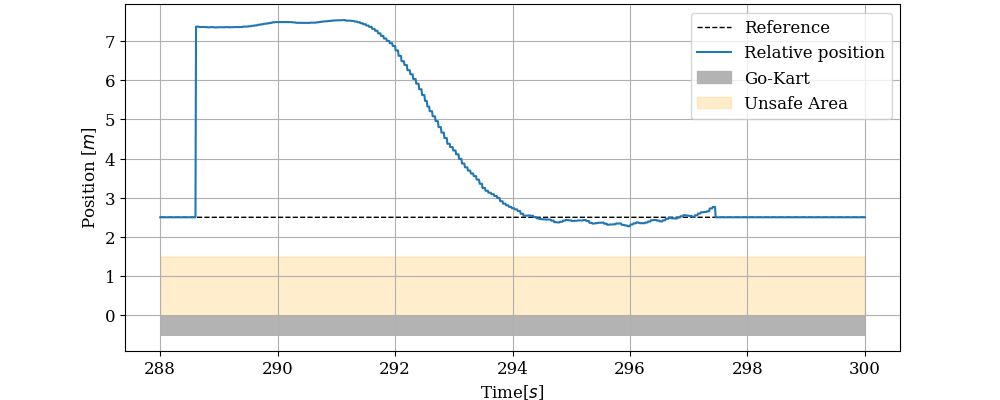
\includegraphics[width=1\textwidth]{Hardware_test/Position} 
	\end{center}
	\vspace{-0.4cm}
	\begin{center}
  		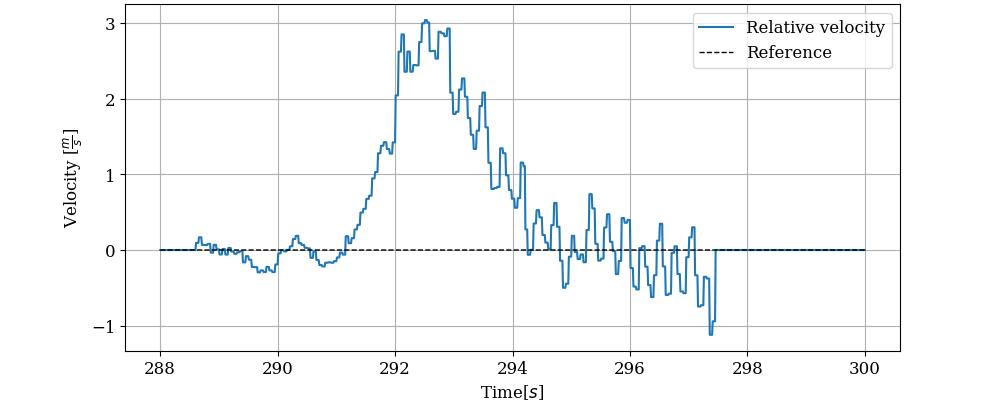
\includegraphics[width=1\textwidth]{Hardware_test/Velocity} 
	\end{center}
	\vspace{-0.4cm}
	\begin{center}
  		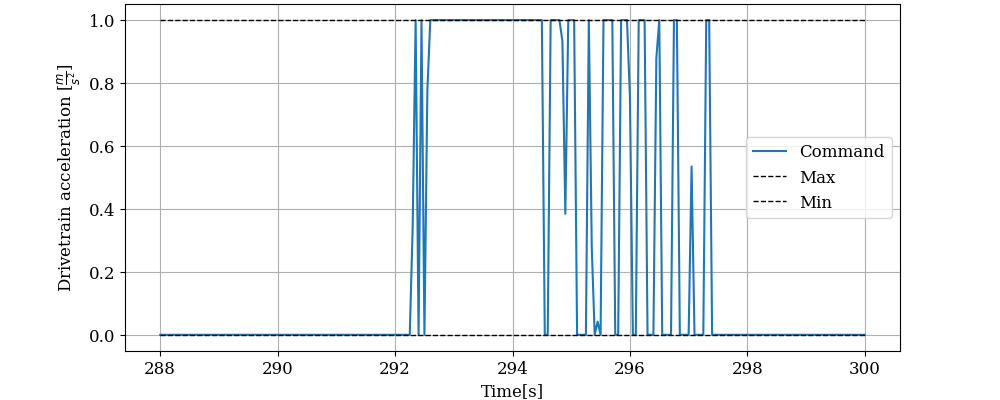
\includegraphics[width=1\textwidth]{Hardware_test/Input} 
	\end{center}
\end{column}

\begin{column}{0.6\textwidth}
\vspace{-0.4cm}
\begin{block}{}
\centering
\textcolor{red}{Oscillations around steady state condition, especially in the input variable}
\end{block}
\vspace{0.2cm}
	\begin{center}
  		\onslide<2,3>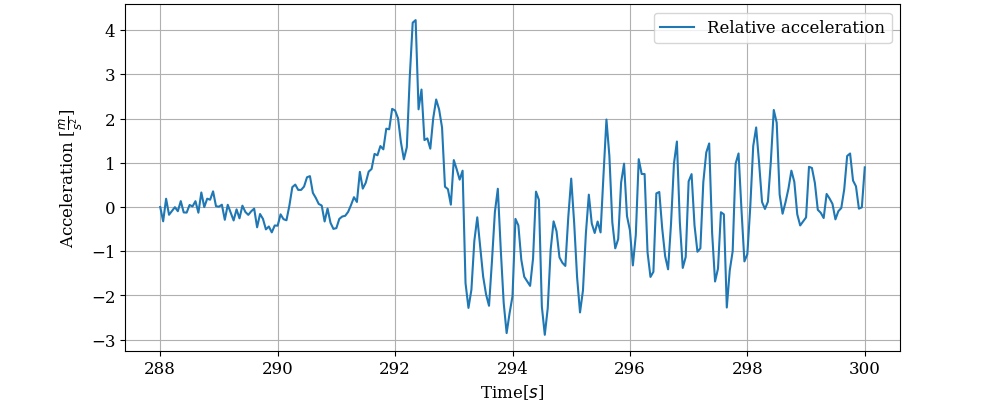
\includegraphics[width=0.8\textwidth]{Hardware_test/Acceleration} 
	\end{center}

\onslide<3>The system results reliable in the usage on the track and field racetrack

\vspace{0.1cm}
\onslide<3>\begin{block}{}
Runner absolute acceleration estimation can be improved by:
\begin{itemize}
	\footnotesize
	\item[$\blacktriangleright$] adding an IMU on the runner's body 
	\item[$\blacktriangleright$] introducing a learning approach
\end{itemize}
\end{block}

\end{column}
\end{columns}

\end{frame}

%%%%%% TA-LOU SIMULATION %%%%%%%%%%%%%%%%%%%%%%%%%%%%%%%%%%%%%%%%%%%%%%%%%%%%%%%%%%%
\begin{frame}
\frametitle{Female athlete simulation results - Controllers comparison}
\begin{columns}
\begin{column}{0.57\textwidth}
\centering
\begin{block}{}
\centering
Test the three controllers on the same velocity profile \\
mimic the one of a female professional athlete during a competition.
\end{block}
\vspace{-0.2cm}
\begin{block}{}
\textbf{Initial distance:}
\centering
$\Delta p_\text{init} = d_\text{des} + \bar{d}, \quad \bar{d}=4$m
\end{block}
	\begin{center}
  		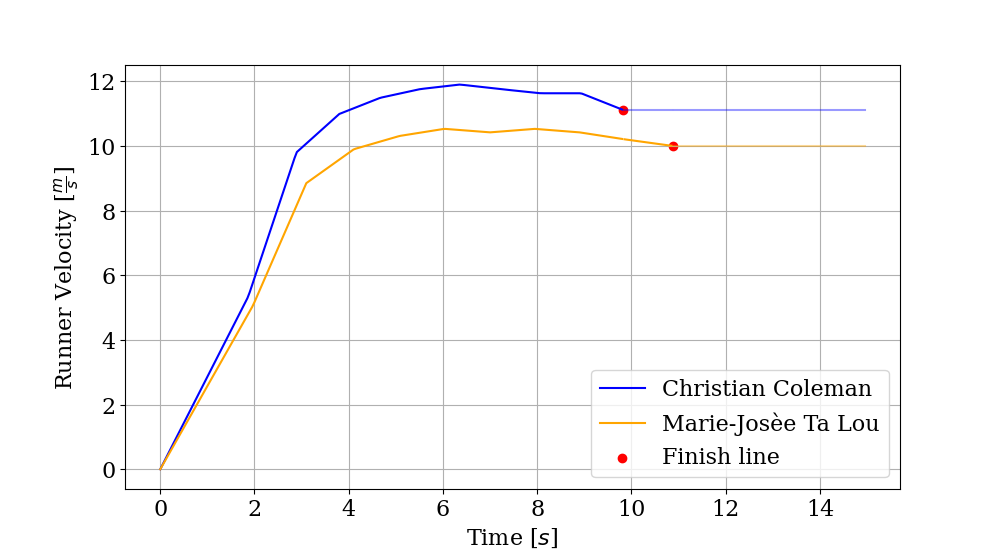
\includegraphics[width=0.6\textwidth]{Test_Velocities_back} 
	\end{center}
	\begin{center}
  		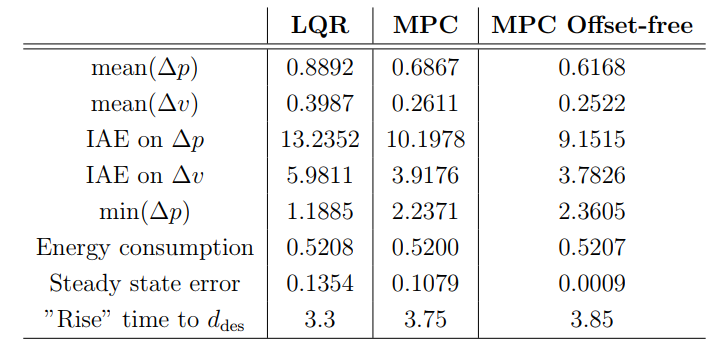
\includegraphics[width=0.7\textwidth]{Ta_Lou/Table} 
	\end{center}

\end{column}
\begin{column}{0.43\textwidth}
	\begin{center}
  		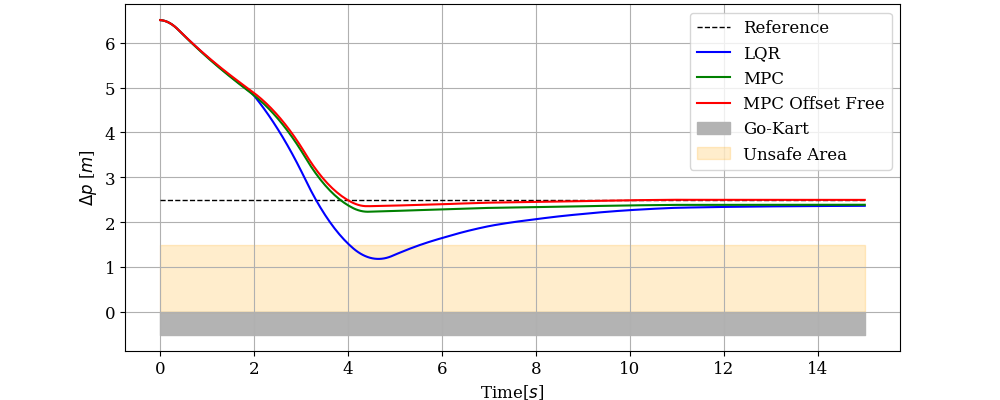
\includegraphics[width=1\textwidth]{Ta_Lou/Deltap} 
	\end{center}
	\vspace{-0.4cm}
	\begin{center}
  		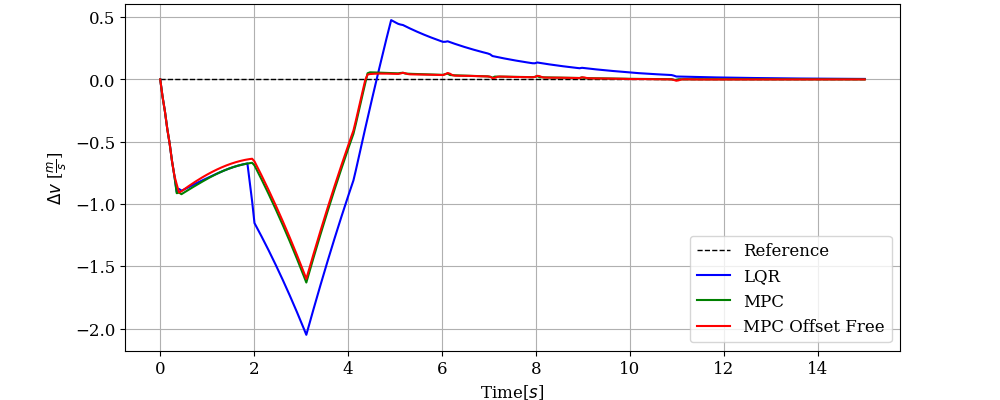
\includegraphics[width=1\textwidth]{Ta_Lou/Deltav} 
	\end{center}
	\vspace{-0.4cm}
	\begin{center}
  		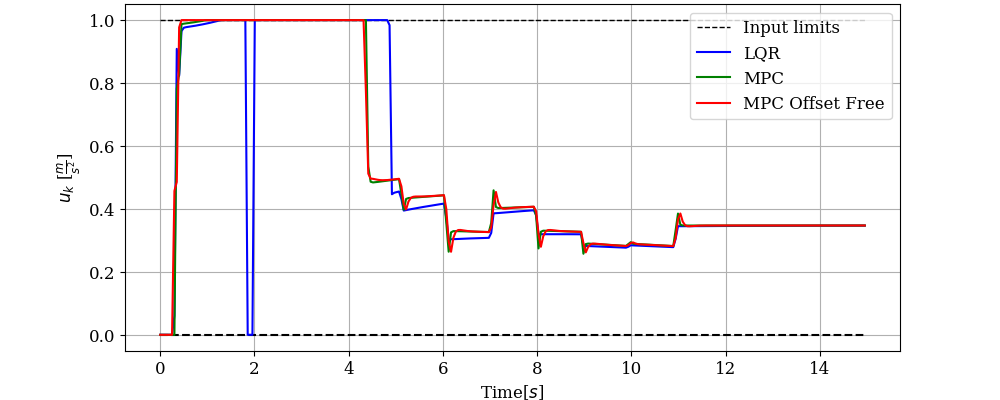
\includegraphics[width=1\textwidth]{Ta_Lou/Input} 
	\end{center}
\end{column}
\end{columns}
\end{frame}


%%%%%% COLEMAN SIMULATION %%%%%%%%%%%%%%%%%%%%%%%%%%%%%%%%%%%%%%%%%%%%%%%%%%%%%%%%%
\begin{frame}
\frametitle{Male athlete simulation results - Controllers comparison}
\begin{columns}
\begin{column}{0.57\textwidth}
\centering
\begin{block}{}
\centering
Test the three controllers on the same velocity profile \\
mimic the one of a male professional athlete during a competition.
\end{block}
\vspace{-0.2cm}
\begin{block}{}
\textbf{Initial distance:}
\centering
$\Delta p_\text{init} = d_\text{des} + \bar{d}, \quad \bar{d}= 13$m
\end{block}
	\begin{center}
  		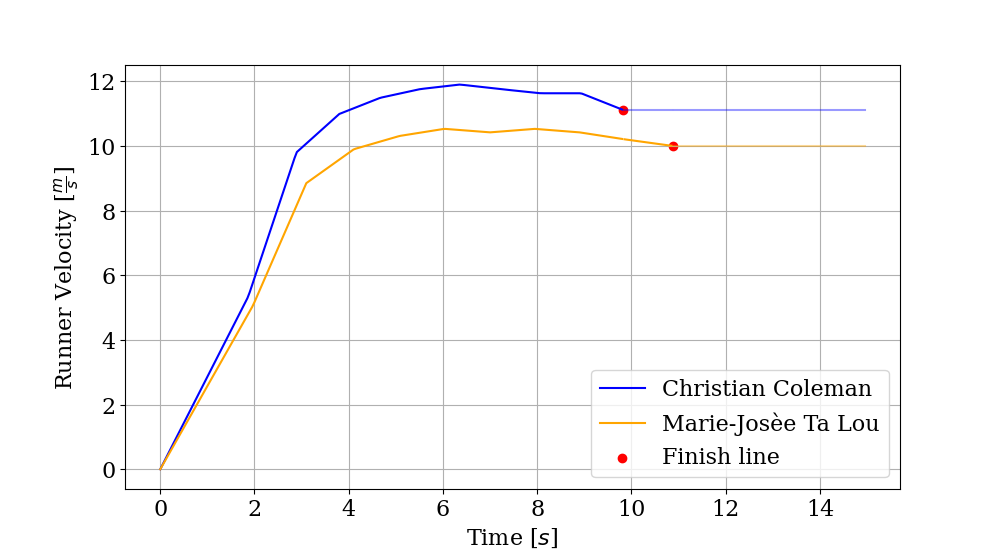
\includegraphics[width=0.6\textwidth]{Test_Velocities_back} 
	\end{center}
	\begin{center}
  		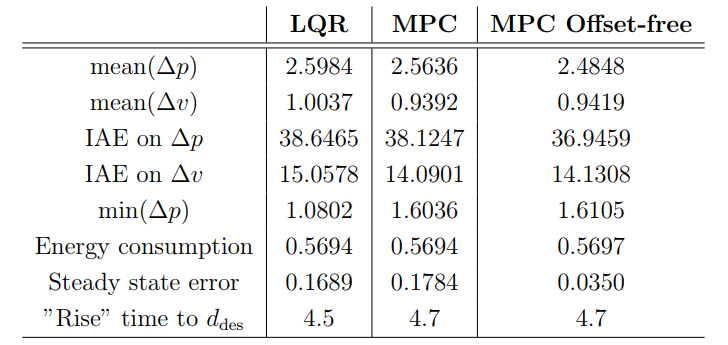
\includegraphics[width=0.7\textwidth]{Coleman/Table} 
	\end{center}

\end{column}
\begin{column}{0.43\textwidth}
	\begin{center}
  		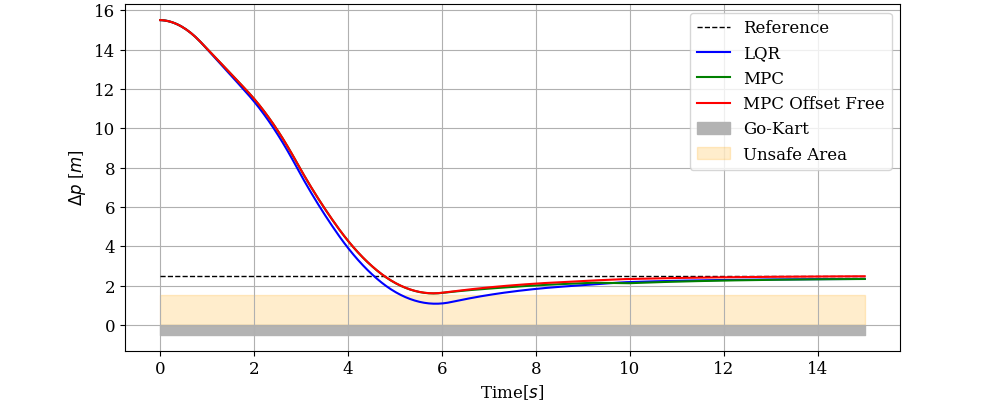
\includegraphics[width=1\textwidth]{Coleman/Deltap} 
	\end{center}
	\vspace{-0.4cm}
	\begin{center}
  		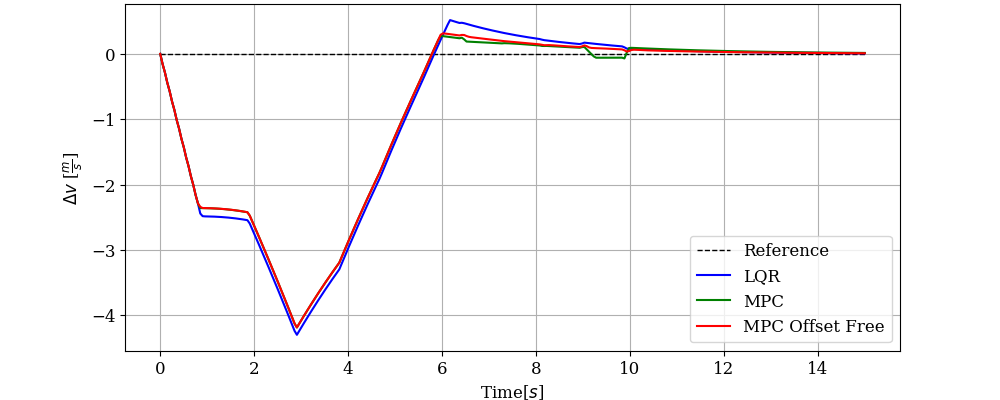
\includegraphics[width=1\textwidth]{Coleman/Deltav} 
	\end{center}
	\vspace{-0.4cm}
	\begin{center}
  		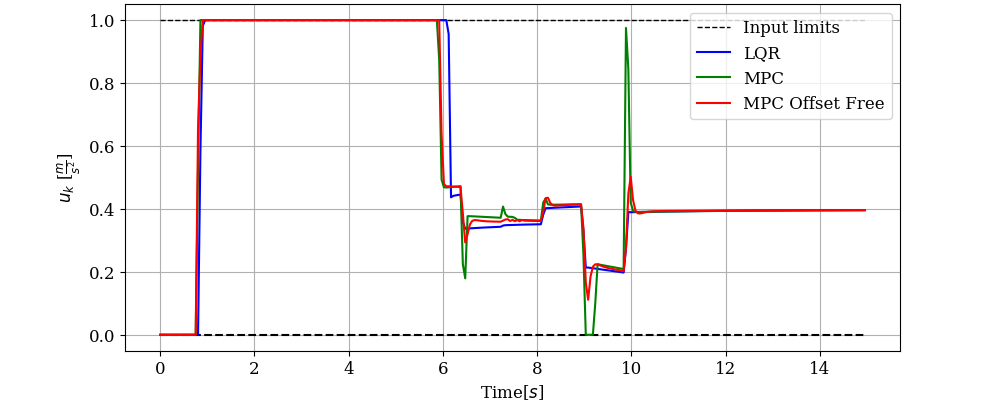
\includegraphics[width=1\textwidth]{Coleman/Input} 
	\end{center}
\end{column}
\end{columns}
\end{frame}

%%%%%% COMPUTATIONAL EFFORT %%%%%%%%%%%%%%%%%%%%%%%%%%%%%%%%%%%%%%%%%%%%%%%%%%%%%%%%
\begin{frame}
\frametitle{Controllers computational effort}
\begin{columns}
\begin{column}{0.22\textwidth}
\begin{block}{}
	\begin{center}
  		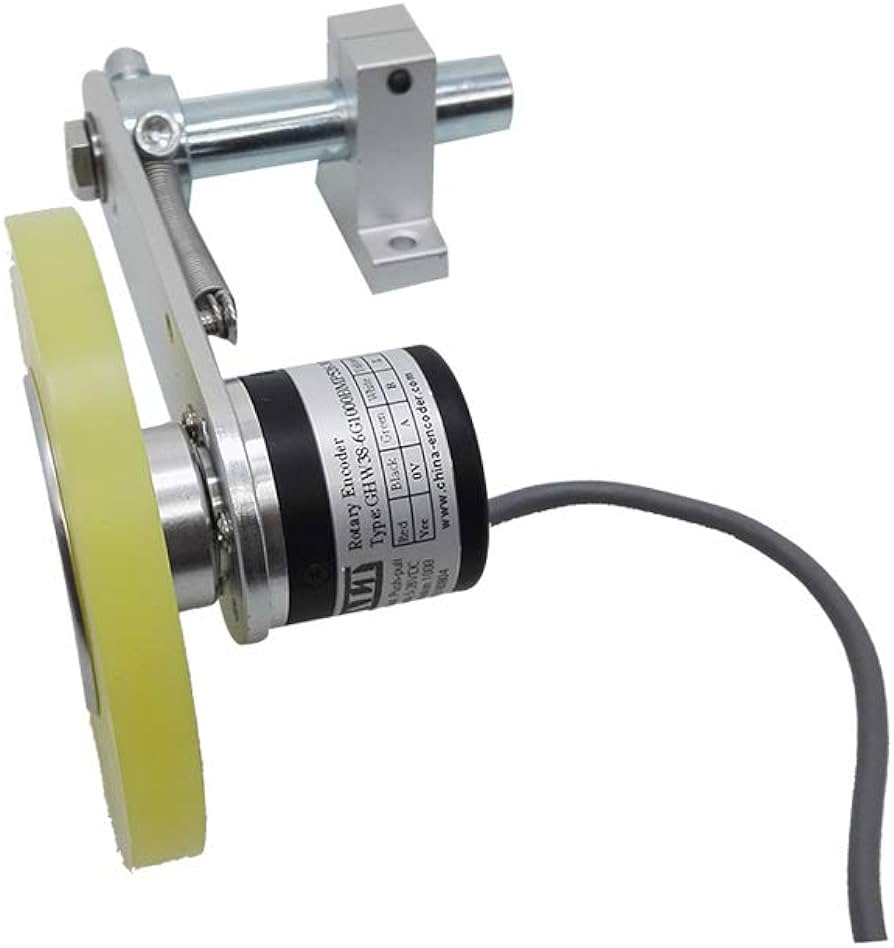
\includegraphics[width=0.25\textwidth]{Wheel_Encoder} 
	\end{center}
\centering
\textbf{Wheel Encoders} \\
Frequency: 100 Hz \\
Sampling time: 10 ms
\end{block}
\end{column}

\begin{column}{0.22\textwidth}
\begin{block}{}
	\begin{center}
  		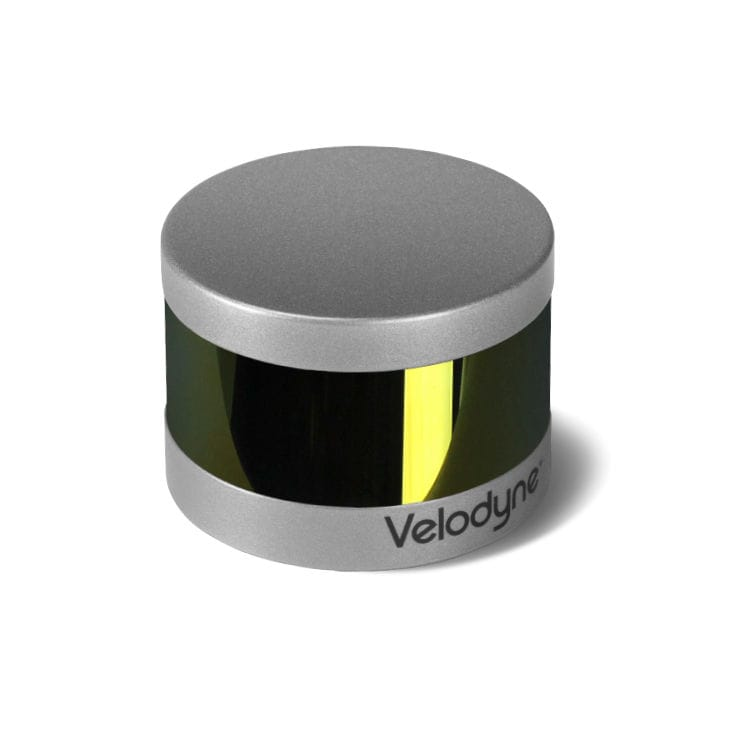
\includegraphics[width=0.25\textwidth]{Lidar} 
	\end{center}
\centering
\textbf{LiDAR (Velodyne)} \\
Frequency: 20 Hz \\
Sampling time: 50 ms
\end{block}
\end{column}


\begin{column}{0.22\textwidth}
\begin{block}{}
	\begin{center}
  		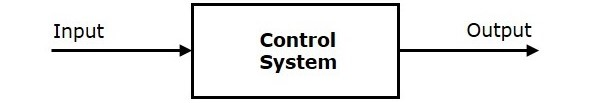
\includegraphics[width=1\textwidth]{Control} 
	\end{center}
\centering
\textbf{Controller} \\
Frequency: 20 Hz \\
Sampling time: 50 ms
\end{block}
\end{column}

\begin{column}{0.22\textwidth}
\begin{block}{}
	\begin{center}
  		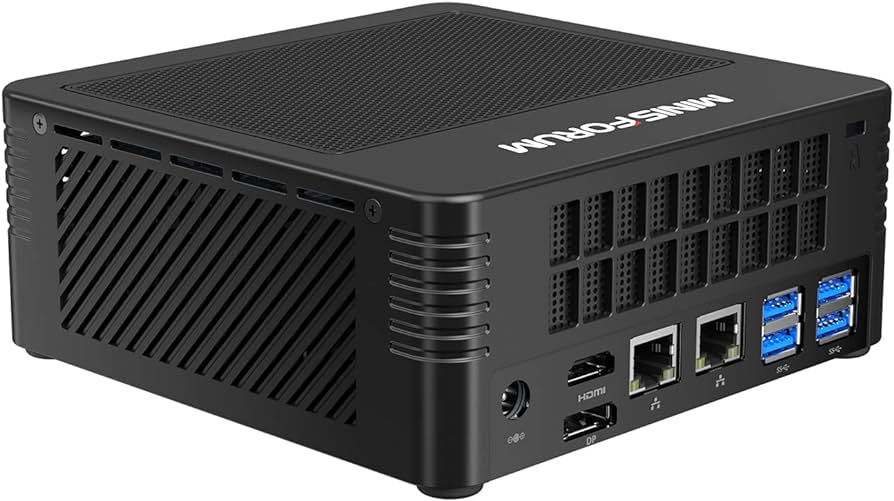
\includegraphics[width=0.3\textwidth]{PC} 
	\end{center}
\centering
\textbf{Computer board} \\
AMD Ryzen 7 5700G  \\
Frequency: 3.8 GHz 
\end{block}
\end{column}
\end{columns}

\vspace{0.4cm}
\begin{columns}
\begin{column}{0.6\textwidth}
\centering
Controllers computational required efforts \\
computed in the Python Simulation Environment
	\begin{center}
  		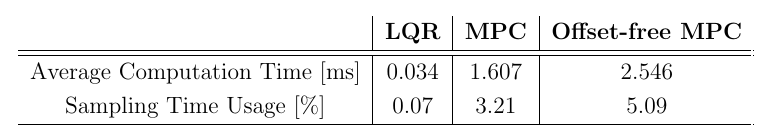
\includegraphics[width=1\textwidth]{Table_back} 
	\end{center}
\end{column}

\begin{column}{0.4\textwidth}
	\begin{center}
  		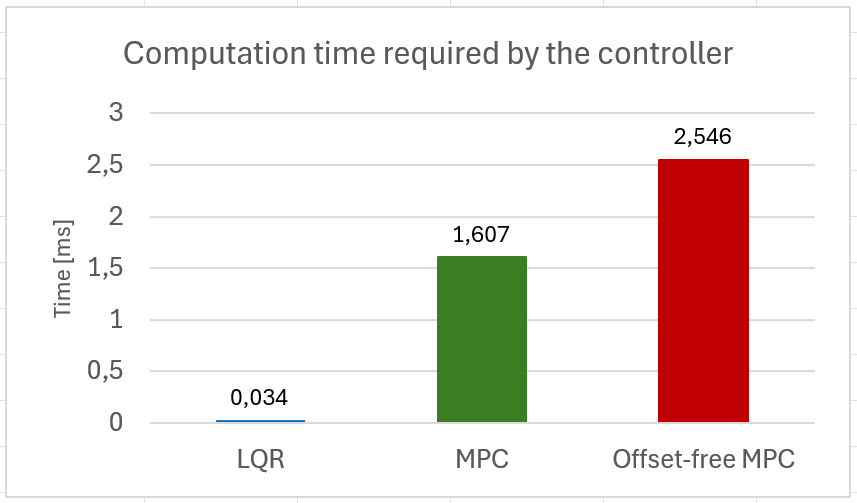
\includegraphics[width=1\textwidth]{Effort} 
	\end{center}
\end{column}
\end{columns}
\end{frame}


%%%%%% GO-KART REPOSITORY %%%%%%%%%%%%%%%%%%%%%%%%%%%%%%%%%%%%%%%%%%%%%%%%%%%%%%%%%
\begin{frame}
\frametitle{Go-kart repository for hardware implementation}
\begin{columns}
\begin{column}{0.35\textwidth}
	\begin{center}
  		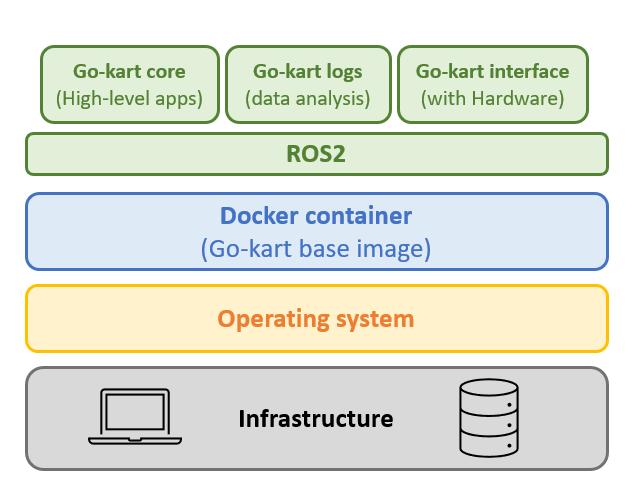
\includegraphics[width=1\textwidth]{Repo}
	\end{center}
\end{column}
\begin{column}{0.7\textwidth}
\centering
The repo is composed of four different docker images
\vspace{0.2cm}
\begin{itemize}
	\footnotesize
	\item[$\blacktriangleright$] \textbf{Base image}: Ubuntu 20.04, ROS 2 and communication with other images
	\item[$\blacktriangleright$] \textbf{Go-kart logs}: Data analysis (from binary data to csv files)	
	\item[$\blacktriangleright$] \textbf{Go-kart interface}: Interface with hardware components (actuators and sensors)
	\item[$\blacktriangleright$] \textbf{Go-kart core}: High level applications (estimation, control, visualization, ecc)
\end{itemize}
\end{column}
\end{columns}

\begin{columns}
\begin{column}{0.6\textwidth}

\end{column}
\begin{column}{0.1\textwidth}
	\begin{center}
  		
\includegraphics[width=1\textwidth]{ROS2}
	\end{center}
\end{column}
\hspace{-0.6cm}
\begin{column}{0.1\textwidth}
	\begin{center}
  		
\includegraphics[width=0.8\textwidth]{Docker} 
	\end{center}
\end{column}
\hspace{-0.6cm}
\begin{column}{0.1\textwidth}
	\begin{center}
  		
\includegraphics[width=0.7\textwidth]{Python}
	\end{center}
\end{column}
\hspace{-0.6cm}
\begin{column}{0.1\textwidth}
	\begin{center}
  		
\includegraphics[width=0.9\textwidth]{GitHub} 
	\end{center}
\end{column}
\end{columns}
\end{frame}


%%%%%% STATE ESTIMATOR and DISTURBANCE OBSERVER %%%%%%%%%%%%%%%%%%%%%%%%%%%%%%%%%%%%%%%%%%%

\backupend



\end{document}



